% RevTeX4-2 working note
\documentclass[aps,prb,onecolumn,nofootinbib,superscriptaddress]{revtex4-2}

\usepackage{amsmath,amssymb,amsthm,mathtools,bm}
\usepackage{booktabs}
\usepackage{graphicx}
\usepackage{xcolor}
\usepackage[colorlinks=true,linkcolor=blue,citecolor=blue,urlcolor=blue]{hyperref}
\hypersetup{bookmarksdepth=2}
\usepackage{microtype}
% Permit compilation from form_factor_analysis/, its docs/ directory, or the repo root.
\graphicspath{{figs/}{../figs/}{form_factor_analysis/figs/}}

\newtheorem{proposition}{Proposition}

\newcommand{\mc}[1]{\mathcal{#1}}
\newcommand{\mb}[1]{\mathbb{#1}}
\newcommand{\mbf}[1]{\mathbf{#1}}
\newcommand{\bs}[1]{\boldsymbol{#1}}
\newcommand{\ket}[1]{\left|#1\right\rangle}
\newcommand{\bra}[1]{\left\langle#1\right|}
\newcommand{\braket}[2]{\left\langle#1\,\middle|\,#2\right\rangle}
\newcommand{\ev}[2]{\left\langle#2\,\middle|\,#1\,\middle|\,#2\right\rangle}
\newcommand{\norm}[1]{\left\lVert#1\right\rVert}

\begin{document}

\title{Effect of Real-Space Truncation on the Overcomplete Wannier Form-Factor Obstruction}

\author{Asadullah Bhuiyan}
\date{\today}

\begin{abstract}
We analyze how a finite-support truncation of an overcomplete Wannier (OW) measurement mode changes the overlap form factor by which it probes a Chern band.  The untruncated form factor of a band with Chern number $C\neq0$ necessarily has zeros whose winding records the band obstruction.  A real-space window produces a twisted momentum-space convolution, and the relevant question for the adaptive circuit is whether the resulting overlap $f_n^{\mathrm{eff}}(\mbf{k})$ retains this zero and winding.  We distinguish three length scales which must not be conflated: the root-mean-square OW spread $\xi_{\mathrm{rms}}$, its topological lower bound $\xi_{\mathrm{top}}=\sqrt{2|C|}\,\ell$, and the asymptotic exponential tail length $\xi_{\mathrm{exp}}$.  For the $\alpha=1$ model and the $X$-trial mode used in the code, $\xi_{\mathrm{top}}\simeq0.564a$, $\xi_{\mathrm{rms}}\simeq0.674a$, and $\xi_{\mathrm{exp}}\simeq1.443a$.  Direct computation for the square $n_{\mathrm{shell}}$ mask shows that $n_{\mathrm{shell}}=1$ retains $99.2155\%$ of the OW norm and preserves the displaced overlap zero with its winding.  Finally, we explain why this overlap-winding statement is distinct from assigning a nonzero Fukui--Hatsugai--Suzuki Chern number to the normalized finite-support spinor itself: a smooth, periodic, nowhere-vanishing compact-support spinor is a global section and therefore has trivial Chern class.
\end{abstract}

\maketitle
\setcounter{tocdepth}{2}
\tableofcontents

%%%%%%%%%%%%%%%%%%%%%%%%%%%%%%%%%%%%%%%%%%%%%%%%%%%%%
\section{Setup and Definitions}
\label{sec:setup}
%%%%%%%%%%%%%%%%%%%%%%%%%%%%%%%%%%%%%%%%%%%%%%%%%%%%%

Consider a single isolated band with Bloch states $\ket{\psi_{\mbf{k}}}$ and cell-periodic part $\ket{u_{\mbf{k}}}$, normalized so that $\braket{u_{\mbf{k}}}{u_{\mbf{k}}} = 1$. Let $\ket{\tau}$ be a smooth, normalized trial spinor (we specialize to a $\mbf{k}$-independent trial state for clarity; the generalization is immediate) and define the form factor
\begin{equation}
f(\mbf{k}) = \braket{u_{\mbf{k}}}{\tau}.
\end{equation}
The coherent Wannier state centered at lattice site $\mbf{R}$ is
\begin{equation}\label{eq:coherent}
\ket{\chi_{\mbf{R}}} = \frac{1}{\sqrt{N}} \sum_{\mbf{k} \in \mathrm{BZ}} e^{-i\mbf{k}\cdot\mbf{R}}\, f(\mbf{k})\, \ket{\psi_{\mbf{k}}},
\end{equation}
which is exponentially localized since $f(\mbf{k})\ket{\psi_{\mbf{k}}} = P_{\mbf{k}}\ket{\tau}$ is smooth and periodic. The Chern number is given by the phase winding of $f(\mbf{k})$~\cite{Li2024}:
\begin{equation}\label{eq:chern_winding}
C = -\frac{1}{2\pi i} \oint_{\mathrm{BZ}} d\mbf{k} \cdot \nabla_{\mbf{k}} \ln f(\mbf{k}).
\end{equation}
The in-band projection of the trial state is $P_-(\mbf{k})\ket{\tau} = f(\mbf{k})\ket{u_{\mbf{k}}}$, so $f(\mbf{k})$ is also the overlap amplitude between the projected trial spinor and the lower-band eigenvector.

\paragraph*{Connection to the overcomplete Wannier circuit.} In the adaptive Markov circuit studied in the companion code, the parameter \texttt{nshell} specifies precisely the real-space support radius of the overcomplete Wannier (OW) measurement modes. An OW mode centered at $\mbf{R}$ is constructed by projecting the trial spinor $\ket{\tau}$ with the band projector, then retaining only real-space sites $\mbf{r}$ satisfying $|d_x(\mbf{r},\mbf{R})|\leq n_{\mathrm{shell}}$ and $|d_y(\mbf{r},\mbf{R})|\leq n_{\mathrm{shell}}$ (or the nearest-neighbor cross for $n_{\mathrm{shell}}=1/2$). The present analysis identifies this truncation as a real-space multiplication $g(\mbf{r})=g_n(\mbf{r})$ acting on the coherent state, and the form factor of the truncated mode is precisely $f_n^{\mathrm{eff}}$ derived below.

%%%%%%%%%%%%%%%%%%%%%%%%%%%%%%%%%%%%%%%%%%%%%%%%%%%%%
\section{General Real-Space Modulation}
\label{sec:general}
%%%%%%%%%%%%%%%%%%%%%%%%%%%%%%%%%%%%%%%%%%%%%%%%%%%%%

\subsection{Definition and effective form factor}

Let $g(\mbf{r})$ be an arbitrary complex-valued function on the lattice. We define the modulated state
\begin{equation}\label{eq:modulated}
\ket{\Phi^{(g)}} = g(\hat{\mbf{r}}) \ket{\chi_{\mbf{R}}},
\end{equation}
where the multiplication is diagonal in the real-space basis:
$\Phi^{(g)}(\mbf{r}) = g(\mbf{r})\,\chi_{\mbf{R}}(\mbf{r}).$
Writing $g$ in terms of its Fourier transform,
\begin{equation}\label{eq:g_fourier}
g(\mbf{r}) = \frac{1}{N}\sum_{\mbf{q}} \tilde{g}(\mbf{q})\, e^{i\mbf{q}\cdot\mbf{r}},
\end{equation}
and substituting \eqref{eq:coherent}, we project onto the Bloch state $\ket{\psi_{\mbf{k}'}}$ to define the \emph{effective form factor}:
\begin{equation}\label{eq:feff_def}
f^{(g)}(\mbf{k}') := \sqrt{N}\, e^{i\mbf{k}'\cdot\mbf{R}}\braket{\psi_{\mbf{k}'}}{\Phi^{(g)}}.
\end{equation}
Computing the inner product using $\braket{\psi_{\mbf{k}'}}{\psi_{\mbf{k}}} = \delta_{\mbf{k}',\mbf{k}}$ on a finite lattice yields the central formula:
\begin{equation}\label{eq:feff_general}
\boxed{f^{(g)}(\mbf{k}') = \frac{1}{N}\sum_{\mbf{k} \in \mathrm{BZ}} \tilde{g}(\mbf{k}'-\mbf{k})\, e^{-i(\mbf{k}'-\mbf{k})\cdot\mbf{R}}\, f(\mbf{k})\, \braket{u_{\mbf{k}'}}{u_{\mbf{k}}}.}
\end{equation}
Several remarks are in order.
\begin{itemize}
\item \textbf{Twisted convolution.} $f^{(g)}$ is a convolution of $f(\mbf{k})$ with $\tilde{g}$, dressed by the Bloch state overlap $\braket{u_{\mbf{k}'}}{u_{\mbf{k}}}$ and a phase factor $e^{-i(\mbf{k}'-\mbf{k})\cdot\mbf{R}}$ that encodes the center of the coherent state.

\item \textbf{Flat-band limit.} If $\ket{u_{\mbf{k}}}$ is $\mbf{k}$-independent, the overlap is unity and the effective form factor reduces to a standard (phased) convolution:
\begin{equation}\label{eq:flat_band}
f^{(g)}(\mbf{k}') \big|_{\text{flat}} = \frac{1}{N}\sum_{\mbf{k}} \tilde{g}(\mbf{k}'-\mbf{k})\, e^{-i(\mbf{k}'-\mbf{k})\cdot\mbf{R}}\, f(\mbf{k}).
\end{equation}

\item \textbf{Normalization independence.} Normalizing $\ket{\Phi^{(g)}}$ replaces $f^{(g)} \to f^{(g)}/\norm{\Phi^{(g)}}$, an overall positive real rescaling. Since a positive constant contributes nothing to the phase winding, define the \emph{overlap-winding index}
\begin{equation}\label{eq:Cg}
\nu_g := \frac{1}{2\pi i}\oint_{\mathrm{BZ}} d\mbf{k}\cdot\nabla_{\mbf{k}}\ln f^{(g)}(\mbf{k}) .
\end{equation}
It is independent of the normalization of $\ket{\Phi^{(g)}}$.  For the unwindowed band form factor, Eq.~\eqref{eq:chern_winding} gives $\nu_0=-C$.  For a windowed state, $\nu_g$ diagnoses the winding of its overlap with the target Chern band; it is not, in general, the Chern number of the windowed real-space state.

\item \textbf{Out-of-band weight.} The component of $\ket{\Phi^{(g)}}$ orthogonal to the band is $Q\ket{\Phi^{(g)}}$, where $Q = 1 - P$ is the complement projector. It is given by the same expression \eqref{eq:feff_general} with $\braket{u_{\mbf{k}'}}{u_{\mbf{k}}}$ replaced by inter-band overlaps $\braket{u^{(n)}_{\mbf{k}'}}{u_{\mbf{k}}}$ for bands $n \neq 1$.
\end{itemize}

\subsection{Topology of the modulated state}
\label{sec:topology}

\subsubsection{Vanishing of the overlap winding when $f^{(g)}$ is nowhere zero}

\noindent\textbf{Lemma 1.} \emph{If $f^{(g)}(\mbf{k})$ is continuous and nowhere vanishing on $T^2$, then $\nu_g = 0$.}

\medskip
\noindent\emph{Proof.} If $f^{(g)}(\mbf{k}) \neq 0$ for all $\mbf{k}$, then the map $\mbf{k} \mapsto f^{(g)}(\mbf{k})/|f^{(g)}(\mbf{k})|$ defines a continuous map $T^2 \to S^1$. The total vorticity enclosed by a fundamental Brillouin-zone cell is
\begin{equation}
\nu_g = \frac{1}{2\pi i}\oint d\mbf{k}\cdot\nabla_{\mbf{k}}\ln f^{(g)}(\mbf{k}) = \frac{1}{2\pi}\oint d\mbf{k}\cdot\nabla_{\mbf{k}}\arg f^{(g)}(\mbf{k})
\end{equation}
and, because there are no zeros in the cell, contributions from opposite boundary edges cancel pairwise by periodicity:
\begin{equation}
\nu_g = \frac{1}{2\pi}\left[\int_0^1 dk_1\,\partial_{k_1}\arg f^{(g)}\big|_{k_2=1} - \int_0^1 dk_1\,\partial_{k_1}\arg f^{(g)}\big|_{k_2=0}\right] = 0.
\end{equation}
Thus there is no net zero vorticity enclosed by the Brillouin-zone torus.  This statement does not forbid independent noncontractible $S^1$ windings of a nowhere-vanishing complex scalar along individual cycles of $T^2$; those are not the Chern-obstruction index considered here. $\square$

\subsubsection{Preservation of zeros: narrow $\tilde{g}$}

\noindent\textbf{Lemma 2.} \emph{Suppose $f(\mbf{k})$ has a zero of order $|C|$ and winding $-C$ at $\mbf{k}_0$, with $f(\mbf{k}_0 + \mbf{q}) \approx A_0(q_x - i\,\mathrm{sgn}(C)\,q_y)^{|C|}$ for $|\mbf{q}| \leq \delta k$. Let $\tilde{g}$ satisfy $|\tilde{g}(\mbf{q})| \leq \epsilon$ for $|\mbf{q}| > \Lambda$ with $\Lambda \ll \delta k$. Then $f^{(g)}$ has a zero near $\mbf{k}_0$ with the same winding, provided $\epsilon$ is sufficiently small.}

\medskip
\noindent\emph{Proof.} We temporarily work in the flat-band limit; the general case follows since the overlap deviates from $\delta_{\mbf{k}',\mbf{k}}$ by $O(|\mbf{k}'-\mbf{k}|) = O(\Lambda)$. In this limit, $f^{(g)}(\mbf{k}')$ is a phased convolution
\begin{equation}\label{eq:fg_conv}
f^{(g)}(\mbf{k}') = \frac{1}{N}\sum_{\mbf{k}} \tilde{g}(\mbf{k}'-\mbf{k})\,e^{-i(\mbf{k}'-\mbf{k})\cdot\mbf{R}}\, f(\mbf{k}).
\end{equation}
Define $h(\mbf{k}) = \tilde{g}(\mbf{k})e^{-i\mbf{k}\cdot\mbf{R}}$; then $f^{(g)} = (1/N)(h * f)$.

Consider a circle $\gamma_\rho$ of radius $\rho$ around $\mbf{k}_0$ with $\Lambda \ll \rho \ll \delta k$. On $\gamma_\rho$, $|f(\mbf{k}_0 + \mbf{q})| \sim |A_0|\rho^{|C|}$. Splitting the convolution correction into $|\mbf{q}| \leq \Lambda$ and $|\mbf{q}| > \Lambda$:
\begin{equation}
|f^{(g)}(\mbf{k}) - f(\mbf{k})| \lesssim |A_0|\,|C|\,\rho^{|C|-1}\Lambda + \epsilon\norm{f}_\infty.
\end{equation}
For $\rho \gg \Lambda$ and $\epsilon$ small, both terms are $\ll |A_0|\rho^{|C|} \sim |f(\mbf{k})|$ on $\gamma_\rho$. By Rouch\'{e}'s theorem, $f^{(g)}$ and $f$ have the same zeros counted with winding inside $\gamma_\rho$, giving $\nu_g=\nu_0=-C$. $\square$

\subsubsection{Destruction of zeros: broad $\tilde{g}$}

\noindent\textbf{Lemma 3.} \emph{Suppose $f(\mbf{k})$ has a zero at $\mbf{k}_0$ with $|f(\mbf{k}_0 + \mbf{q})| \lesssim |A_0||\mbf{q}|^{|C|}$ for $|\mbf{q}| \leq \delta k$, and $|f(\mbf{k})| \geq f_{\min} > 0$ for $|\mbf{k} - \mbf{k}_0| \geq \delta k$. Let $|h(\mbf{q})| = |\tilde{g}(\mbf{q})e^{-i\mbf{q}\cdot\mbf{R}}|$ be smooth with $|h(\mbf{q})| \geq h_0 > 0$ for $|\mbf{q}| \leq \Lambda$ and $\Lambda \gg \delta k$. Then $f^{(g)}(\mbf{k}_0) \neq 0$ generically.}

\medskip
\noindent\emph{Proof.} Evaluate \eqref{eq:fsig_k0} in the flat-band limit, decomposing into the zero region $Z = \{|\mbf{q}|\leq\delta k\}$ and its complement:
\begin{equation}\label{eq:case2_decomp}
f^{(g)}(\mbf{k}_0) = \underbrace{\frac{1}{N}\sum_{|\mbf{q}|\leq\delta k} h(\mbf{q})\,f(\mbf{k}_0+\mbf{q})}_{I_Z} + \underbrace{\frac{1}{N}\sum_{|\mbf{q}|>\delta k} h(\mbf{q})\,f(\mbf{k}_0+\mbf{q})}_{I_{Z^c}}.
\end{equation}
One finds $|I_Z| = O(\sigma^2(\delta k)^{|C|+2})$ while $|I_{Z^c}| = O(\sigma^2 f_{\min})$ generically (i.e., absent fine-tuned phase cancellation in $I_{Z^c}$). Since $(\delta k)^{|C|+2}/|\mbf{b}|^2 \ll 1$, we have $|I_Z|/|I_{Z^c}| \to 0$ and $f^{(g)}(\mbf{k}_0) \neq 0$. $\square$

\medskip
\noindent\textbf{Remark.} The word ``generically'' cannot be removed: one can always construct pathological $g$ (e.g., $g=0$) producing fine-tuned cancellations. The content of Lemma~3 is that for $g$ drawn from any reasonable parametric family, the zero is filled once the kernel width exceeds $\delta k$, except on a measure-zero set of parameters.

\subsubsection{Three distinct localization scales}

The spread entering the quantum-geometric bound is the second moment of the unwindowed OW coherent state,
\begin{equation}\label{eq:xirms_def}
\xi_{\mathrm{rms}}^2 := \ev{\mbf{r}^{\,2}}{\chi_{\mbf{R}=0}} .
\end{equation}
The Li--Dong--Ledwith--Khalaf bound states
\begin{equation}\label{eq:top_spread_bound}
\xi_{\mathrm{rms}} \geq \xi_{\mathrm{top}},
\qquad
\xi_{\mathrm{top}}:=\sqrt{2|C|}\,\ell,
\qquad
2\pi\ell^2=A_{\mathrm{uc}},
\qquad
\ell^2=\frac{2\pi}{A_{\mathrm{BZ}}},
\end{equation}
where $A_{\mathrm{uc}}A_{\mathrm{BZ}}=(2\pi)^2$.  For a square lattice with $A_{\mathrm{uc}}=a^2$ and $|C|=1$, this lower bound is
\begin{equation}
\xi_{\mathrm{top}}=\frac{a}{\sqrt{\pi}}\simeq0.564\,a .
\end{equation}
The zero-resolution momentum scale may be estimated parametrically by $\delta k=O(\xi_{\mathrm{rms}}^{-1})$, so a window broad in real space compared with the actual OW spread gives a narrow convolution kernel.  This is a scale estimate, not a theorem that a window of radius $\xi_{\mathrm{top}}$ preserves a particular zero.

A second, independent length is the asymptotic tail-decay scale $\xi_{\mathrm{exp}}$, defined from the large-distance envelope
\begin{equation}
\norm{\chi_{\mbf{0}}(\mbf{r})}\sim e^{-|\mbf{r}|/\xi_{\mathrm{exp}}}
\quad (|\mbf{r}|\to\infty),
\end{equation}
up to algebraic prefactors.  It controls small discarded tails rather than the RMS weight or the survival of the overlap-winding singularity.  In particular, $\xi_{\mathrm{exp}}>\xi_{\mathrm{rms}}$ does not imply that a compact window whose radius is below $\xi_{\mathrm{exp}}$ destroys the form-factor zero.

%%%%%%%%%%%%%%%%%%%%%%%%%%%%%%%%%%%%%%%%%%%%%%%%%%%%%
\section{Specialization: Box Function of Radius \texorpdfstring{$\sigma$}{sigma}}
\label{sec:box}
%%%%%%%%%%%%%%%%%%%%%%%%%%%%%%%%%%%%%%%%%%%%%%%%%%%%%

We now specialize to the circular box (indicator) function
\begin{equation}\label{eq:box_def}
g(\mbf{r}) = B_\sigma(\mbf{r} - \mbf{R}') := \begin{cases} 1 & |\mbf{r} - \mbf{R}'| \leq \sigma \\ 0 & |\mbf{r} - \mbf{R}'| > \sigma \end{cases},
\end{equation}
whose Fourier transform is
\begin{equation}\label{eq:box_FT}
\tilde{g}(\mbf{q}) = \widetilde{B}_\sigma(\mbf{q})\,e^{-i\mbf{q}\cdot\mbf{R}'}, \qquad \widetilde{B}_\sigma(\mbf{q}) = \frac{2\pi\sigma}{|\mbf{q}|}\,J_1(|\mbf{q}|\sigma),
\end{equation}
with $J_1$ the Bessel function of the first kind. The central lobe has width $\Delta k \sim 1/\sigma$, but $\widetilde{B}_\sigma$ has oscillating power-law tails $\sim |\mbf{q}|^{-3/2}$ at large $|\mbf{q}|$. Substituting into \eqref{eq:feff_general} and defining $\bs{\Delta}=\mbf{R}'-\mbf{R}$:
\begin{equation}\label{eq:feff_box2}
\boxed{f_\sigma(\mbf{k}') = e^{-i\mbf{k}'\cdot\bs{\Delta}}\,\frac{1}{N}\sum_{\mbf{k}} \widetilde{B}_\sigma(\mbf{k}'-\mbf{k})\, e^{i\mbf{k}\cdot\bs{\Delta}}\, f(\mbf{k})\,\braket{u_{\mbf{k}'}}{u_{\mbf{k}}}.}
\end{equation}
The overall phase $e^{-i\mbf{k}'\cdot\bs{\Delta}}$ has zero winding and drops out of $\nu_\sigma$. When $\bs{\Delta}=0$ (box centered on the coherent state), \eqref{eq:feff_box2} reduces to the twisted convolution of $f$ with $\widetilde{B}_\sigma$, dressed by the Bloch overlap.

\subsection*{Power-law tails of \texorpdfstring{$\widetilde{B}_\sigma$}{B-sigma}}

Unlike a smooth window (Gaussian, etc.) whose Fourier transform is rapidly decaying, $\widetilde{B}_\sigma(\mbf{q})$ has power-law tails $\sim |\mbf{q}|^{-3/2}\cos(|\mbf{q}|\sigma - 3\pi/4)$. This means the box convolution mixes momenta over \emph{all} scales, albeit with decreasing weight. The dominant contribution still comes from $|\mbf{q}| \lesssim 1/\sigma$, so comparison with $\xi_{\mathrm{rms}}$ remains a useful parametric estimate. However, the tails imply that the crossover between preserved and removed overlap winding is less sharp than for a smooth window.

%%%%%%%%%%%%%%%%%%%%%%%%%%%%%%%%%%%%%%%%%%%%%%%%%%%%%
\section{Gradient Expansion for \texorpdfstring{$\sigma \gg a$}{sigma much greater than a}}
\label{sec:gradient}
%%%%%%%%%%%%%%%%%%%%%%%%%%%%%%%%%%%%%%%%%%%%%%%%%%%%%

Restricting to the centered case $\mbf{R}'=\mbf{R}$ and expanding \eqref{eq:feff_box2} for $\sigma \gg a$ (lattice spacing), we use the moments of the box kernel ($\int \mbf{q}\,\widetilde{B}_\sigma(\mbf{q}) = 0$ by radial symmetry; $\int q_\mu q_\nu\,\widetilde{B}_\sigma(\mbf{q}) = \frac{\delta_{\mu\nu}}{4}\sigma^{-2}$) and expand the Bloch overlap to second order:
\begin{align}
\braket{u_{\mbf{k}'}}{u_{\mbf{k}'+\mbf{q}}} &= 1 - i A_\mu(\mbf{k}') q_\mu - \frac{1}{2}\left[g_{\mu\nu}(\mbf{k}') + i\frac{1}{2}\epsilon_{\mu\nu}\Omega(\mbf{k}')\right]q_\mu q_\nu + O(q^3),
\end{align}
where $A_\mu = i\braket{u_{\mbf{k}}}{\partial_{k_\mu} u_{\mbf{k}}}$ is the Berry connection, $g_{\mu\nu} = \mathrm{Re}\,\braket{\partial_{k_\mu}u_{\mbf{k}}}{Q_{\mbf{k}}\partial_{k_\nu}u_{\mbf{k}}}$ is the quantum metric, and $\Omega$ is the Berry curvature. The result is
\begin{equation}\label{eq:fsigma_expansion}
f_\sigma(\mbf{k}) = (f * \widetilde{B}_\sigma)(\mbf{k}) - i A_\mu(\mbf{k})\,(\partial_{k_\mu}f * \widetilde{B}_\sigma)(\mbf{k}) + O(\sigma^{-2}).
\end{equation}
The leading term is a scalar convolution; the first correction involves the Berry connection and is suppressed by $O(1/\sigma)$.

%%%%%%%%%%%%%%%%%%%%%%%%%%%%%%%%%%%%%%%%%%%%%%%%%%%%%
\section{Zeros of \texorpdfstring{$f_\sigma$}{f-sigma} and the Overlap-Winding Index}
\label{sec:zeros}
%%%%%%%%%%%%%%%%%%%%%%%%%%%%%%%%%%%%%%%%%%%%%%%%%%%%%

We specialize to the centered case $\mbf{R}'=\mbf{R}$, so that
\begin{equation}\label{eq:fsig_recall}
f_\sigma(\mbf{k}') = \frac{1}{N}\sum_{\mbf{k}} \widetilde{B}_\sigma(\mbf{k}'-\mbf{k})\, f(\mbf{k})\,\braket{u_{\mbf{k}'}}{u_{\mbf{k}}}.
\end{equation}
Following Ref.~\cite{Li2024}, the zeros of $f(\mbf{k})$ can be arranged in the single-zero (SZ) gauge where there is a single zero at $\mbf{k}_0$ with
\begin{equation}\label{eq:f_zero}
f(\mbf{k}_0 + \mbf{q}) = A_0 (q_x - i\,\mathrm{sgn}(C)\, q_y)^{|C|} + R(\mbf{q}),
\end{equation}
where $A_0 \neq 0$ and $R(\mbf{q}) = O(|\mbf{q}|^{|C|+1})$.

\subsection{Case 1: \texorpdfstring{$\sigma \gg \xi_{\mathrm{rms}}$}{sigma much greater than xi-rms} --- preservation of zeros}

\noindent\textbf{Proposition (Case 1).} \emph{Let $\sigma \gg \xi_{\mathrm{rms}}$ and $\widetilde{B}_\sigma$ be the Fourier transform of a circular box of radius $\sigma$. If the convolved overlap is a sufficiently small perturbation of $f$ on a loop surrounding $\mbf{k}_0$, then $f_\sigma$ has a zero near $\mbf{k}_0$ with winding $-C$, so that $\nu_\sigma=-C$.}

\medskip
\noindent\emph{Proof.}
\textit{Step 1: Decomposition.} Write \eqref{eq:fsig_recall} at $\mbf{k}'=\mbf{k}_0$ as
\begin{equation}\label{eq:fsig_k0}
f_\sigma(\mbf{k}_0) = \frac{1}{N}\sum_{\mbf{q}} \widetilde{B}_\sigma(\mbf{q})\, f(\mbf{k}_0 + \mbf{q})\,\braket{u_{\mbf{k}_0}}{u_{\mbf{k}_0+\mbf{q}}},
\end{equation}
decomposed into near ($|\mbf{q}|\leq\rho$) and far ($|\mbf{q}|>\rho$) regions with $1/\sigma \ll \rho \ll \delta k$.

\textit{Step 2: Leading near-region harmonic.} Using the leading zero structure \eqref{eq:f_zero} and passing to polar coordinates:
\begin{equation}\label{eq:angular_integral}
I_{\text{near}} \propto \int_0^\rho q\,dq\,\widetilde{B}_\sigma(q)\,q^{|C|} \underbrace{\int_0^{2\pi}\frac{d\phi_q}{2\pi}\, e^{-i|C|\phi_q}}_{= 0 \text{ for } |C|\geq 1} = 0.
\end{equation}
The displayed leading harmonic integrates to zero against a radial kernel.  Subleading terms from $R(\mbf{q})$ and from the Bloch-overlap factor need not vanish exactly; rather, in the narrow-kernel regime they are perturbative and can shift the zero away from $\mbf{k}_0$ without changing its winding.

\textit{Step 3: Winding stability.} For $|\mbf{q}|>\rho\gg 1/\sigma$, the kernel is in its asymptotic tail regime $|\widetilde{B}_\sigma(\mbf{q})| \lesssim C_B\,\sigma^{1/2}\,|\mbf{q}|^{-3/2}$. Applying Rouch\'{e}'s theorem on a circle $\gamma_\rho$ of radius $\rho$ around $\mbf{k}_0$ whenever the total correction is smaller than $|f|$ on that circle establishes that $f_\sigma$ has the same number of zeros with the same winding as $f$ inside $\gamma_\rho$, hence $\nu_\sigma=-C$. $\square$

\subsection{Case 2: \texorpdfstring{$\sigma \ll \xi_{\mathrm{rms}}$}{sigma much less than xi-rms} --- destruction of zeros}

\noindent\textbf{Proposition (Case 2).} \emph{Let $\sigma \ll \xi_{\mathrm{rms}}$. Then generically $f_\sigma(\mbf{k}_0) \neq 0$; if no replacement zero is generated elsewhere on $T^2$, the overlap winding is $\nu_\sigma=0$.}

\medskip
\noindent\emph{Proof.} Direct application of Lemma~3. Since $\sigma \ll \xi_{\mathrm{rms}}$ places the central lobe of $\widetilde{B}_\sigma$ broad compared with the zero-resolution scale, substantial kernel weight enters from outside the zero region. The ratio $|I_Z|/|I_{Z^c}| = O((\delta k)^{|C|+2}/|\mbf{b}|^2) \ll 1$ forces $f_\sigma(\mbf{k}_0) \approx I_{Z^c} \neq 0$ absent symmetry-enforced cancellation. If $f_\sigma$ is nowhere zero after this rearrangement, Lemma~1 gives $\nu_\sigma=0$. $\square$

\subsection{Crossover and the topological bound}

The crossover between Cases~1 and 2 is estimated by comparing the window size with the actual OW spread, so that the central-lobe width $\Delta k=1/\sigma$ resolves the form-factor zero.  The geometric lower bound \eqref{eq:top_spread_bound} implies only the parametric lower scale
\begin{equation}
\boxed{\sigma_{\mathrm{crit}}=O(\xi_{\mathrm{rms}}),
\qquad
\xi_{\mathrm{rms}}\geq\xi_{\mathrm{top}}=\sqrt{2|C|}\,\ell.}
\end{equation}
For $\sigma$ large compared with the relevant spread, overlap winding is stable; for aggressive truncation it may be removed or reorganized.  The inequality constrains the possible OW spread, but does not certify any particular discrete window.  In particular, the survival of the $n_{\mathrm{shell}}=1$ zero must be and is checked directly below.

%%%%%%%%%%%%%%%%%%%%%%%%%%%%%%%%%%%%%%%%%%%%%%%%%%%%%
\section{Multiband Generalization}
\label{sec:multiband}
%%%%%%%%%%%%%%%%%%%%%%%%%%%%%%%%%%%%%%%%%%%%%%%%%%%%%

\subsection{Setup}

Let $\ket{\psi_{n,\mbf{k}}}$, $n=1,\ldots,M$, be the Bloch states of $M$ isolated bands with cell-periodic parts $\ket{u_{n,\mbf{k}}}$. Construct $M$ trial states $\ket{\tau_m}$ and define the $M\times M$ overlap matrix
\begin{equation}\label{eq:F_matrix}
F_{nm}(\mbf{k}) = \braket{u_{n,\mbf{k}}}{\tau_m}.
\end{equation}
The total Chern number of the $M$-band subspace is~\cite{Li2024}
\begin{equation}\label{eq:chern_det}
C = -\frac{1}{2\pi i}\oint_{\mathrm{BZ}} d\mbf{k}\cdot\nabla_{\mbf{k}} \ln \det F(\mbf{k}).
\end{equation}
The multiband coherent states are
\begin{equation}\label{eq:coherent_multi}
\ket{\chi_{m,\mbf{R}}} = \frac{1}{\sqrt{N}}\sum_{\mbf{k}} e^{-i\mbf{k}\cdot\mbf{R}} \sum_{n=1}^{M} F_{nm}(\mbf{k})\ket{\psi_{n,\mbf{k}}}.
\end{equation}

\subsection{Effective overlap matrix and its topology}

Define modulated states $\ket{\Phi^{(g)}_m} = g(\hat{\mbf{r}})\ket{\chi_{m,\mbf{R}}}$ and the \emph{effective overlap matrix}:
\begin{equation}\label{eq:Feff_general}
\boxed{F^{(g)}_{nm}(\mbf{k}') = \frac{1}{N}\sum_{\mbf{k}}\sum_{n'=1}^{M} \tilde{g}(\mbf{k}'-\mbf{k})\,e^{-i(\mbf{k}'-\mbf{k})\cdot\mbf{R}}\, F_{n'm}(\mbf{k})\,\braket{u_{n,\mbf{k}'}}{u_{n',\mbf{k}}}.}
\end{equation}
This is the matrix generalization of \eqref{eq:feff_general}. The determinant overlap-winding index of the modulated states relative to the target subspace is
\begin{equation}\label{eq:Cg_multi}
\nu_g^{(M)} = \frac{1}{2\pi i}\oint_{\mathrm{BZ}} d\mbf{k}\cdot\nabla_{\mbf{k}}\ln\det F^{(g)}(\mbf{k}).
\end{equation}
If the modulated vectors are projected back into and form a nonsingular frame for the target subspace, this winding reproduces the subspace obstruction.  For general real-space-windowed vectors with out-of-band weight it is an overlap diagnostic rather than an independent Chern invariant.  An important structural difference from the single-band case is that $\det F^{(g)}$ is a polynomial in the convolved matrix elements, so zeros can in principle be created or annihilated in pairs by the modulation even at intermediate scales.

In the single-zero gauge, $\det F(\mbf{k}_0+\mbf{q}) \approx A_0(q_x-i\,\mathrm{sgn}(C)\,q_y)^{|C|}$. The narrow-kernel continuity argument applies to $\det F^{(g)}$ when $\sigma\gg\xi_{\mathrm{rms}}$, with the same qualification that the zero may shift while its determinant-overlap winding remains stable.

The critical modulation scale for the multiband case remains
\begin{equation}\label{eq:spread_multi}
\sigma_{\mathrm{crit}} = O(\xi_{\mathrm{rms}}), \qquad \xi_{\mathrm{rms}}\geq \sqrt{2|C|}\,\ell,
\end{equation}
where $C$ is now the total Chern number of the $M$-band subspace.

%%%%%%%%%%%%%%%%%%%%%%%%%%%%%%%%%%%%%%%%%%%%%%%%%%%%%
\section{Computational Example: Square \texorpdfstring{$n_{\mathrm{shell}}$}{n-shell} Mask}
\label{sec:numerical}
%%%%%%%%%%%%%%%%%%%%%%%%%%%%%%%%%%%%%%%%%%%%%%%%%%%%%

The numerical notebook accompanying this note studies the two-band lattice Chern-insulator Hamiltonian
\begin{equation}
h(\mbf{k}) = \hat{\mbf{n}}(\mbf{k})\cdot\bs{\sigma},
\qquad
\mbf{n}(\mbf{k}) = \left(\sin k_x,\,\sin k_y,\,\alpha-\cos k_x-\cos k_y\right),
\qquad
\hat{\mbf{n}}=\frac{\mbf{n}}{|\mbf{n}|},
\end{equation}
with lower-band projector $P_-(\mbf{k}) = (1-\hat{\mbf{n}}(\mbf{k})\cdot\bs{\sigma})/2$. For a normalized trial spinor $\ket{\tau}$, the form-factor amplitude is
\begin{equation}
|f(\mbf{k})|^2 = \bra{\tau}P_-(\mbf{k})\ket{\tau} = \frac{1-\hat{\mbf{n}}(\mbf{k})\cdot\mbf{s}_\tau}{2}, \qquad \mbf{s}_\tau=\bra{\tau}\bs{\sigma}\ket{\tau}.
\end{equation}
For the $X$ trial spinor $\ket{\tau_X}=\frac{1}{\sqrt{2}}\bigl(\begin{smallmatrix}1\\1\end{smallmatrix}\bigr)$ with $\mbf{s}_{\tau_X}=(1,0,0)$:
\begin{equation}
|f_X(\mbf{k})|^2 = \frac{1}{2}\left[1-\frac{\sin k_x}{\sqrt{\sin^2 k_x+\sin^2 k_y+(\alpha-\cos k_x-\cos k_y)^2}}\right].
\end{equation}
A true zero requires $\hat{n}_x=1$, i.e., $\sin k_y=0$, $\alpha-\cos k_x-\cos k_y=0$, $\sin k_x>0$. For $\alpha=1$ this gives
\begin{equation}
\mbf{k}_0/\pi = (0.5,\,0).
\end{equation}

Instead of the circular disk window used for analytic estimates, the project code implements the square real-space mask
\begin{equation}
g_n(\mbf{r}) = \begin{cases}1, & |d_x(\mbf{r},\mbf{R})|\leq n,\quad |d_y(\mbf{r},\mbf{R})|\leq n,\\ 0, & \text{otherwise},\end{cases}
\end{equation}
where $d_x,d_y$ are the periodic lattice distances from the window center $\mbf{R}$. For the special case $n_{\mathrm{shell}}=1/2$, only the five-site cross is kept: $\{(0,0),\,(\pm 1,0),\,(0,\pm 1)\}$. In the thermodynamic, centered case, the Fourier transform of the square mask factorizes into Dirichlet kernels,
\begin{equation}
\widetilde{g}_n(\mbf{q}) = e^{-i\mbf{q}\cdot\mbf{R}}\,D_n(q_x)D_n(q_y),
\qquad
D_n(q) = \sum_{m=-n}^{n}e^{-iqm} = \frac{\sin[(n+\frac{1}{2})q]}{\sin(q/2)},
\end{equation}
and the finite-grid computation evaluates
\begin{equation}
f_n^{\mathrm{eff}}(\mbf{k}') = \frac{1}{N}\sum_{\mbf{k}} \widetilde{g}_n(\mbf{k}'-\mbf{k})\,e^{-i(\mbf{k}'-\mbf{k})\cdot\mbf{R}}\, f(\mbf{k})\,\braket{u_-(\mbf{k}')}{u_-(\mbf{k})}.
\end{equation}
Figure~\ref{fig:exact-form-factor-components} shows the exact form factor and its two spinor components on a $50\times 50$ momentum grid. The true zero at $\mbf{k}/\pi=(0.5,0)$ lies between sampled momenta; the nearest sampled minimum occurs at $\mbf{k}/\pi=(0.48,0)$ with $|f|\simeq 3.14\times 10^{-2}$. Figure~\ref{fig:nshell-real-space-masks} shows the real-space support of the truncation for representative values of $n_{\mathrm{shell}}$.

\subsection{Localization scales and retained norm at \texorpdfstring{$\alpha=1$}{alpha = 1}}
\label{sec:localization-scales}

To compare the finite window with the actual OW mode, we use the same lower-band projector and $X$-trial spinor as in the circuit implementation and set the lattice spacing to $a=1$ for the reported numbers.  Direct Fourier evaluation of $P_-(\mbf{k})\ket{\tau_X}$ gives
\begin{equation}
\xi_{\mathrm{rms}}^2=0.453631\,a^2,
\qquad
\xi_{\mathrm{rms}}=0.673521\,a.
\end{equation}
The nearest complex-momentum singularity of the flattened projector controls the long-distance envelope.  At $\alpha=1$,
\begin{equation}
|\mbf{n}(\mbf{k})|^2
=3-2\cos k_x-2\cos k_y+2\cos k_x\cos k_y .
\end{equation}
For transverse decay, setting $k_x=i\kappa$ and taking the nearest real value $k_y=\pi$ gives
\begin{equation}
5-4\cosh\kappa=0,
\qquad
\kappa=\operatorname{arcosh}\frac54=\log2,
\qquad
\xi_{\mathrm{exp}}=\frac{a}{\log2}=1.442695\,a.
\end{equation}
The three lengths are therefore
\begin{equation}
\begin{array}{c|c|l}
\text{scale} & \text{value at }\alpha=1 & \text{meaning}\\
\hline
\xi_{\mathrm{top}} & 0.564190\,a & \text{topological lower bound on RMS spread}\\
\xi_{\mathrm{rms}} & 0.673521\,a & \text{actual OW second-moment radius}\\
\xi_{\mathrm{exp}} & 1.442695\,a & \text{asymptotic exponential tail length}
\end{array}
\end{equation}
These quantities answer different questions.  In particular, the comparatively long asymptotic tail does not imply that most probability weight lies outside a $3\times3$ window.  Applied to the normalized untruncated OW mode, the square masks retain
\begin{equation}
\begin{array}{c|c|c}
n_{\mathrm{shell}} & \text{support} & \sum_{\mbf{r}\in\mathrm{support}}\norm{\chi_{\mbf{0}}(\mbf{r})}^2\\
\hline
1 & 3\times3 & 0.992155\\
2 & 5\times5 & 0.999137
\end{array}
\end{equation}
of its norm.  Thus $n_{\mathrm{shell}}=1$ removes a small long-distance tail; whether it retains the topological overlap obstruction is determined by the form-factor zero below, not by comparing the cutoff radius with $\xi_{\mathrm{exp}}$ alone.

\begin{figure}[t]
\centering
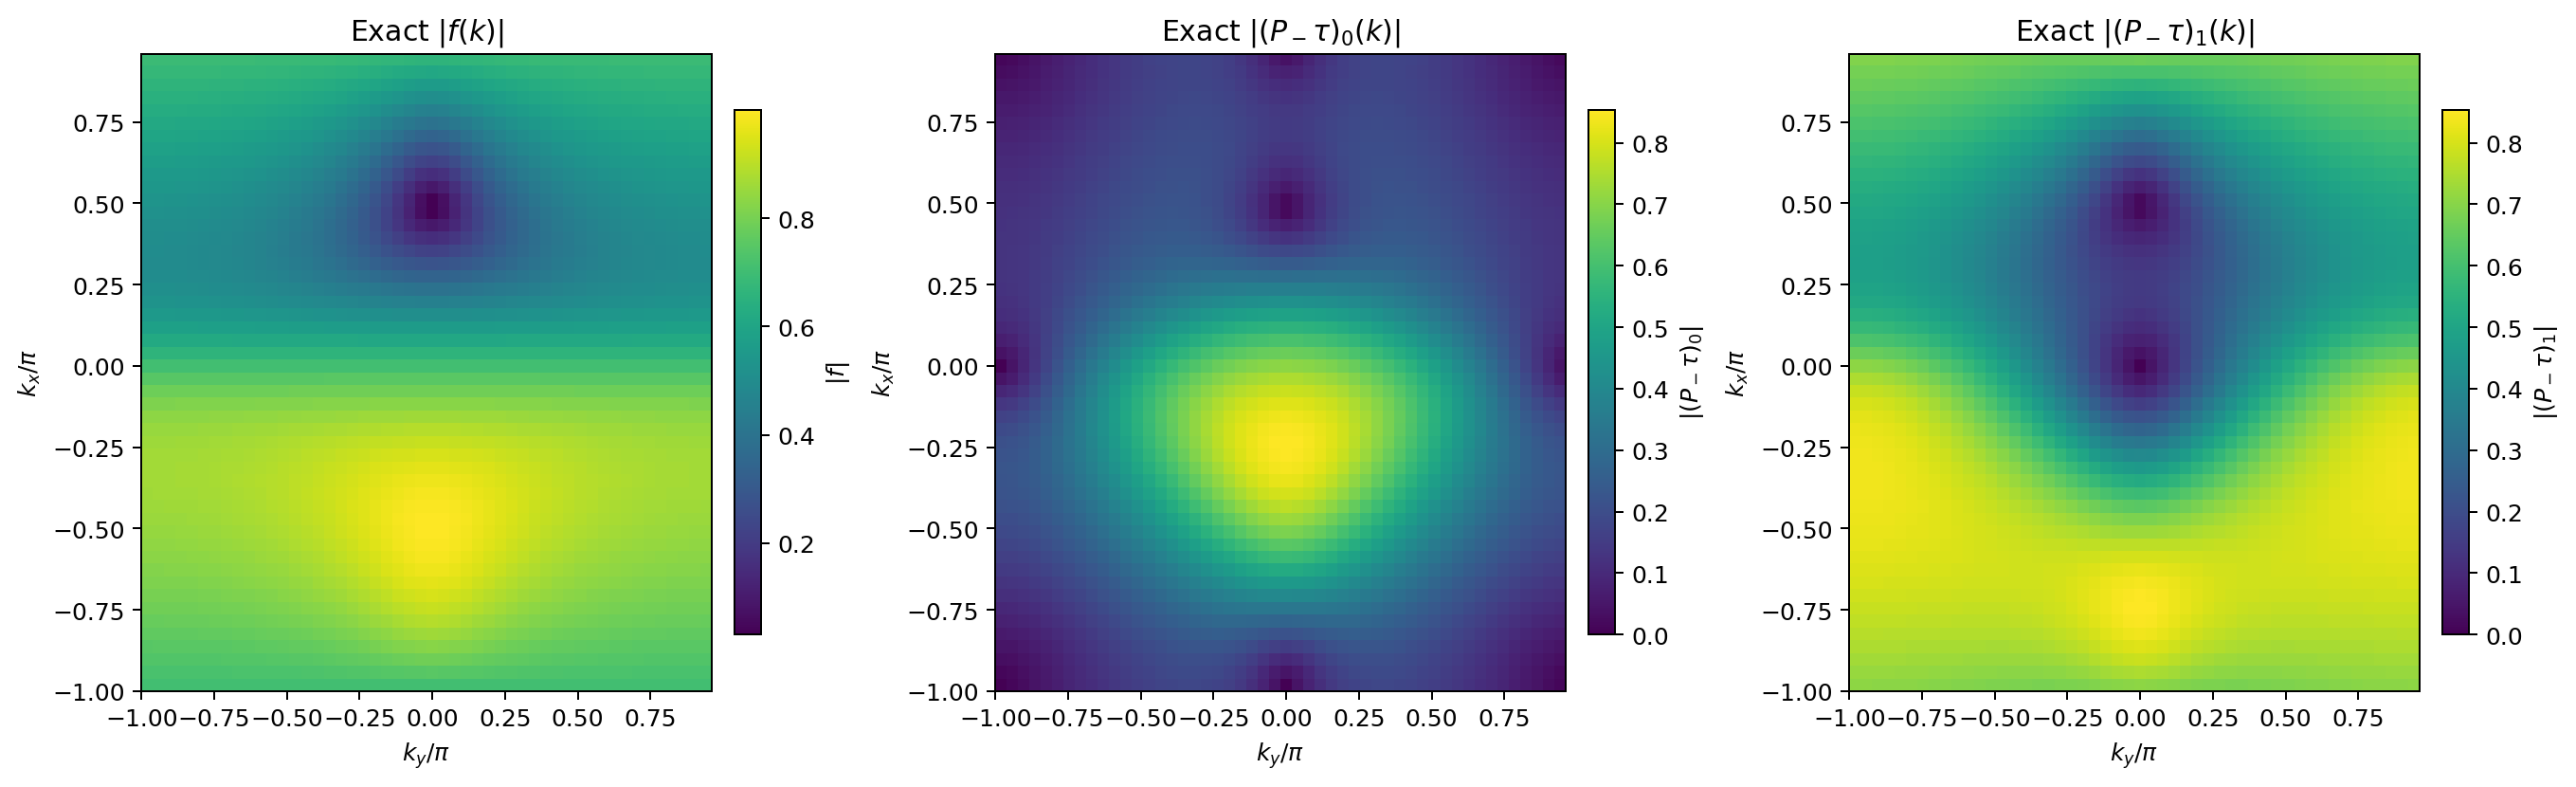
\includegraphics[width=0.85\textwidth]{exact_form_factor_components.png}
\caption{Exact lower-band $X$-trial form factor for the two-band model at $\alpha=1$ on a $50\times 50$ momentum grid. Left: $|f(k)|$, with the true continuum zero at $\mbf{k}/\pi=(0.5,0)$ between sampled momenta. Center and right: the two components of the projected trial state $P_-(\mbf{k})\ket{\tau_X}$.}
\label{fig:exact-form-factor-components}
\end{figure}

\begin{figure}[t]
\centering
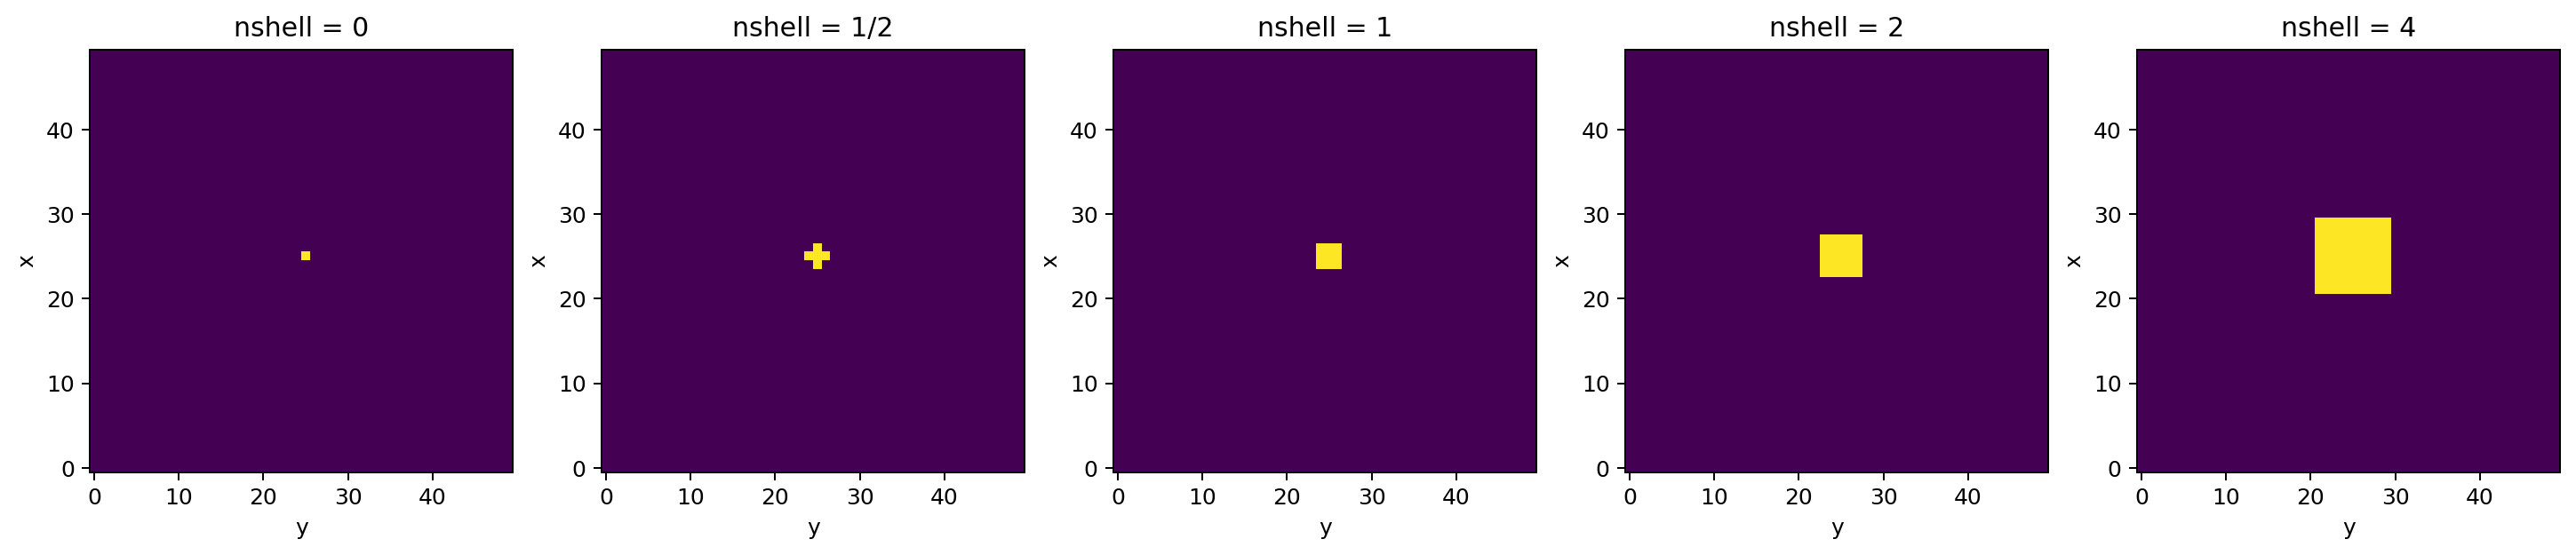
\includegraphics[width=0.85\textwidth]{nshell_real_space_masks.png}
\caption{Real-space square masks used for the finite-$n_{\mathrm{shell}}$ calculation. The $n_{\mathrm{shell}}=0$ case is a single-site mask, hence $\widetilde{g}_0(\mbf{q})$ is flat in momentum space and mixes the whole BZ. Increasing $n_{\mathrm{shell}}$ concentrates the Fourier kernel near $\mbf{q}=0$, enabling a sharper effective form factor.}
\label{fig:nshell-real-space-masks}
\end{figure}

\subsection{The \texorpdfstring{$n_{\mathrm{shell}}=0$}{n-shell = 0} limit}

For $n_{\mathrm{shell}}=0$, the mask reduces to the single site at the origin:
\begin{equation}
g_0(\mbf{r})=\delta_{\mbf{r},\mbf{R}}, \qquad \widetilde{g}_0(\mbf{q})=1 \quad (\text{centered case}).
\end{equation}
Substituting into the effective form factor:
\begin{equation}
f_0^{\mathrm{eff}}(\mbf{k}') = \frac{1}{N}\sum_{\mbf{k}} f(\mbf{k})\,\braket{u_-(\mbf{k}')}{u_-(\mbf{k})}.
\label{eq:feff_nshell0}
\end{equation}
This is a full BZ average of $f(\mbf{k})$ weighted by the Bloch overlap, not a local evaluation of $f$ at $\mbf{k}'$. The original zero of $f$ does not force a zero of $f_0^{\mathrm{eff}}$.

In the continuum limit, only the onsite Fourier coefficient
\begin{equation}
C_{\mbf{0}} = \int_{\mathrm{BZ}}\frac{d^2k}{(2\pi)^2}\,P_-(\mbf{k})
\end{equation}
appears. By the square-lattice symmetries at $\alpha=1$, $C_{\mbf{0}} = \mathrm{diag}(a,\,1-a)$ with $a\simeq 0.254415$, and on the $k_y=0$ line:
\begin{equation}
f_0^{\mathrm{eff}}(k_x,0) = \frac{1}{\sqrt{2}}\left[a\cos\frac{k_x}{2}-(1-a)\sin\frac{k_x}{2}\right].
\end{equation}
This has an accidental zero at $\tan(k_x/2)=a/(1-a)$, i.e.,
\begin{equation}
\mbf{k}_{*,0}/\pi \simeq (0.2093,\,0),
\end{equation}
which is the continuum counterpart of the shallow $50\times 50$ dip near $k_x/\pi=0.20$ ($|f_0^{\mathrm{eff}}|\simeq 8.18\times 10^{-3}$). This is not the topological zero at $k_x/\pi=0.5$: it is an accidental zero of the BZ-averaged object, and it carries the correct winding (see below) only because a zero must exist somewhere on $T^2$ for any state with $C=1$ topology.

\subsection{Explicit checks for \texorpdfstring{$n_{\mathrm{shell}}=1$ and $2$}{n-shell = 1 and 2}}

For $n_{\mathrm{shell}}=1$ (the $3\times 3$ square mask), $D_1(q)=1+2\cos q$ and $\widetilde{g}_1(q_x,q_y)=D_1(q_x)D_1(q_y)$. At $\mbf{k}_0=(\pi/2,0)$, where $\hat{\mbf{n}}(\mbf{k}_0)=(1,0,0)$ and the lower-band spinor is the $-\sigma_x$ eigenstate, one computes
\begin{equation}
f_1^{\mathrm{eff}}(\mbf{k}_0) = -\frac{1}{2N}\sum_{\mbf{k}}(1+2\cos k_y)\frac{1-\cos k_x-\cos k_y}{|\mbf{n}(\mbf{k})|} \simeq -1.21\times 10^{-2},
\end{equation}
so the original zero is displaced from $\mbf{k}_0$. On the symmetry line $k_y=0$, the shifted continuum zero occurs at
\begin{equation}
\mbf{k}_{*,1}/\pi \simeq (0.4922,\,0).
\end{equation}
For $n_{\mathrm{shell}}=2$ (the $5\times 5$ mask), $D_2(q)=1+2\cos q+2\cos 2q$ and similarly
\begin{equation}
f_2^{\mathrm{eff}}(\mbf{k}_0) \simeq -1.17\times 10^{-2}, \qquad \mbf{k}_{*,2}/\pi \simeq (0.4925,\,0).
\end{equation}
In both cases the zero is shifted rather than removed. The shift converges to $k_x/\pi=0.5$ as $n_{\mathrm{shell}}\to\infty$.

\subsection{Persistence of the zero for sufficiently large finite shells}
\label{sec:persistence}

For nonzero $n_{\mathrm{shell}}$, the effective form factor near the original zero at $\mbf{k}_0=(\pi/2,0)$ can be expanded as follows. Write $\mbf{k}'=\mbf{k}_0+\mbf{p}$ and $\mbf{k}=\mbf{k}'+\mbf{q}$. In the centered case $\mbf{R}=0$:
\begin{align}
f_n^{\mathrm{eff}}(\mbf{k}_0+\mbf{p}) &= \frac{A}{N}\sum_{\mbf{q}}\widetilde{g}_n(-\mbf{q})\left[(p_x+q_x)-i(p_y+q_y)\right]+O(\Delta k_n^2) \nonumber\\
&= A\,G_0\,(p_x-ip_y) + \frac{A}{N}\underbrace{\sum_{\mbf{q}}\widetilde{g}_n(-\mbf{q})q_x}_{=0} - \frac{iA}{N}\underbrace{\sum_{\mbf{q}}\widetilde{g}_n(-\mbf{q})q_y}_{=0} + O(\Delta k_n^2),
\label{eq:finite_shell_zero_survival}
\end{align}
where $G_0 = (1/N)\sum_{\mbf{q}}\widetilde{g}_n(-\mbf{q})=g_n(\mbf{0})=1$ and $\Delta k_n\sim 1/(2n+1)$. The first moments vanish because the square mask is inversion-symmetric, $g_n(\mbf{r})=g_n(-\mbf{r})$, making $\widetilde{g}_n(\mbf{q})$ real and even. Therefore,
\begin{equation}
f_n^{\mathrm{eff}}(\mbf{k}_0+\mbf{p}) = A\,(p_x-ip_y)+O(\Delta k_n^2,\,p^2,\,p\Delta k_n),
\end{equation}
and the leading winding structure is identical to the original zero. By a Rouch\'{e}-continuity argument, for sufficiently large $n_{\mathrm{shell}}$ there is a zero of $f_n^{\mathrm{eff}}$ near $\mbf{k}_0$ with the same phase winding.

This is in sharp contrast to the $n_{\mathrm{shell}}=0$ case, where $\widetilde{g}_0$ is completely broad and the small parameter $\Delta k_n$ does not exist.

\subsection{Continuum-\texorpdfstring{$k$}{k} effective form factor cuts}

To go beyond the finite $50\times 50$ sampling grid, we compute the effective spinor state directly from the projector's Fourier coefficients,
\begin{equation}
\ket{\psi_n(\mbf{k})} = \sum_{\mbf{r}\in\mathrm{supp}(g_n)} e^{-i\mbf{k}\cdot\mbf{r}}\,C_{\mbf{r}}\ket{\tau},
\qquad
C_{\mbf{r}} = \int_{\mathrm{BZ}}\frac{d^2q}{(2\pi)^2}\,e^{i\mbf{q}\cdot\mbf{r}}\,P_-(\mbf{q}),
\label{eq:spinor_continuum}
\end{equation}
evaluated on a dense $181\times 181$ momentum grid. The scalar effective form factor is then $f_n^{\mathrm{eff}}(\mbf{k}) = \braket{u_-(\mbf{k})}{\psi_n(\mbf{k})}$, where the lower-band eigenspinor $\ket{u_-(\mbf{k})}$ is determined at each $\mbf{k}$ from a local eigenvector decomposition. This formulation avoids the discrete-grid Fourier artifact of the finite-$N$ computation and yields the true continuum zeros.

Figure~\ref{fig:continuum-ky0-cuts} shows the resulting $k_y=0$ amplitude cuts $|f_n^{\mathrm{eff}}(k_x,0)|$ on the dense continuum grid, and Figure~\ref{fig:continuum-shifted-zeros} shows the same cuts with the shifted zero locations marked explicitly. For $n_{\mathrm{shell}}\geq 1$, the zeros converge toward $k_x/\pi=0.5$ as $n_{\mathrm{shell}}$ increases; for $n_{\mathrm{shell}}=0$, the zero is far displaced to $k_x/\pi\simeq 0.209$.

\begin{figure}[t]
\centering
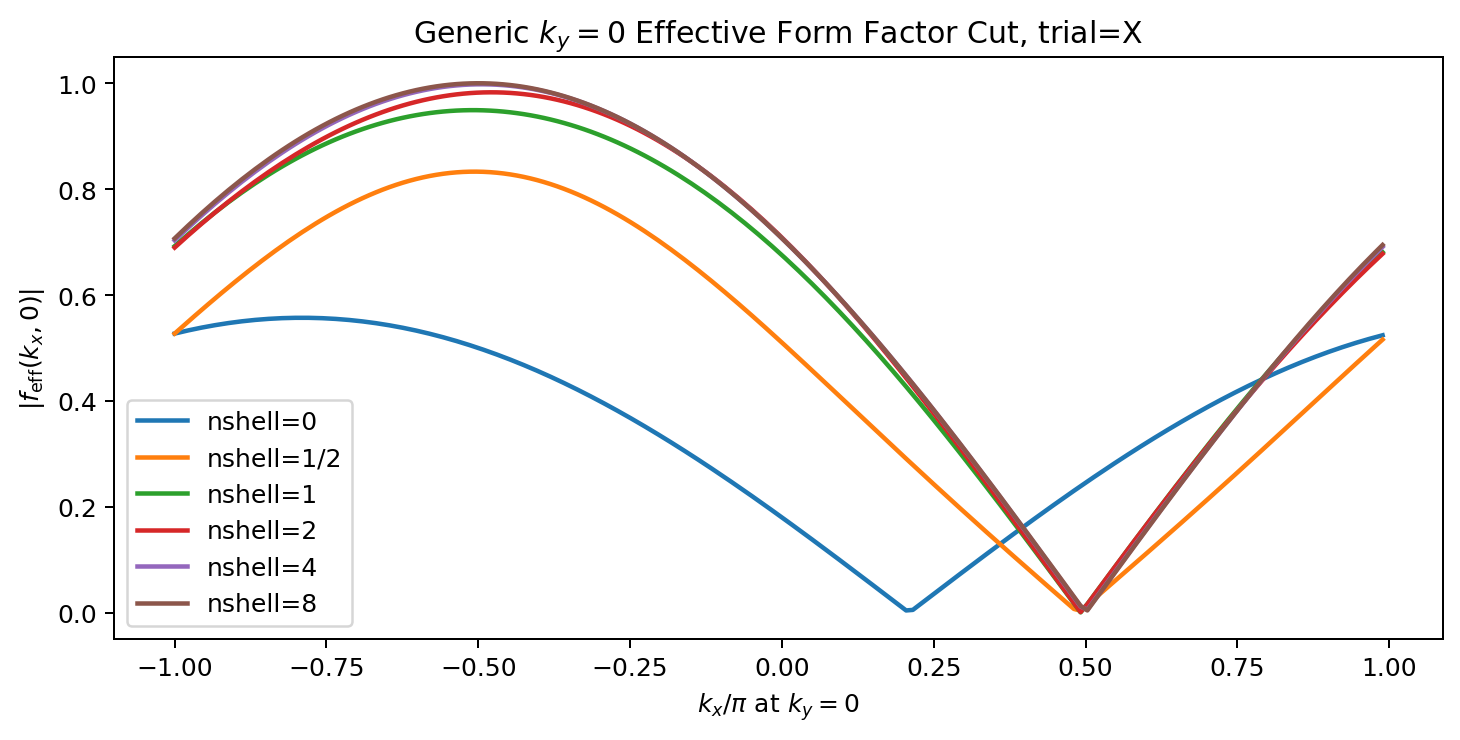
\includegraphics[width=0.75\textwidth]{continuum_generic_ky0_cuts.png}
\caption{Continuum-$\mbf{k}$ cuts of $|f_n^{\mathrm{eff}}(k_x,0)|$ at $k_y=0$ on a $181\times 181$ grid, computed via the projector Fourier coefficients \eqref{eq:spinor_continuum}. Each curve corresponds to a different $n_{\mathrm{shell}}$ value. The minimum for $n_{\mathrm{shell}}=0$ is located far from the original topological zero at $k_x/\pi=0.5$, while the minima for $n_{\mathrm{shell}}\geq 1$ approach $k_x/\pi=0.5$ from below.}
\label{fig:continuum-ky0-cuts}
\end{figure}

\begin{figure}[t]
\centering
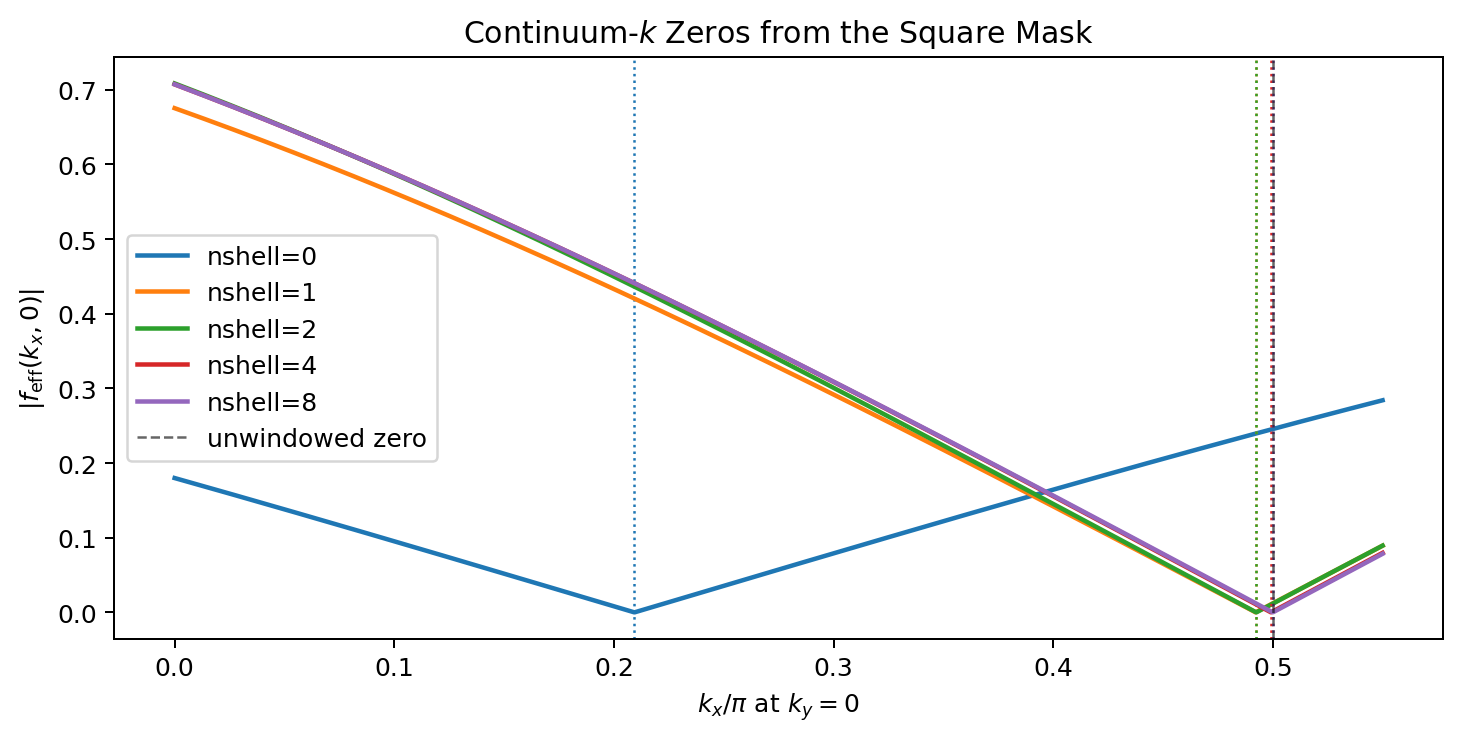
\includegraphics[width=0.82\textwidth]{continuum_shifted_zeros.png}
\caption{Continuum-$k$ cuts of the finite-shell effective form factor on $k_y=0$. The dashed vertical line is the unwindowed zero at $k_x/\pi=0.5$. For $n_{\mathrm{shell}}=0$, the dotted line near $k_x/\pi\simeq 0.209$ is an accidental zero of the fully BZ-averaged onsite truncation. For $n_{\mathrm{shell}}=1,2,4,8$, the dotted lines show the shifted descendants of the unwindowed zero, which converge monotonically toward $k_x/\pi=0.5$.}
\label{fig:continuum-shifted-zeros}
\end{figure}

\subsection{Effective form factor maps and the approach to the unwindowed limit}

The full BZ dependence of $|f_n^{\mathrm{eff}}(\mbf{k})|$ is shown in Figures~\ref{fig:effective-form-factor-maps} and \ref{fig:effective-form-factor-cuts}. As $n_{\mathrm{shell}}$ increases, the effective form factor approaches the unwindowed result: the amplitude maximum rises toward unity (see the printed values $\max|f_n^{\mathrm{eff}}|=0.556,\, 0.988,\, 0.949,\, 0.983,\, 0.998,\, 0.999$ for $n=0,1/2,1,2,4,8$) and the zero approaches the continuum location $\mbf{k}/\pi=(0.5,0)$.

\begin{figure}[t]
\centering
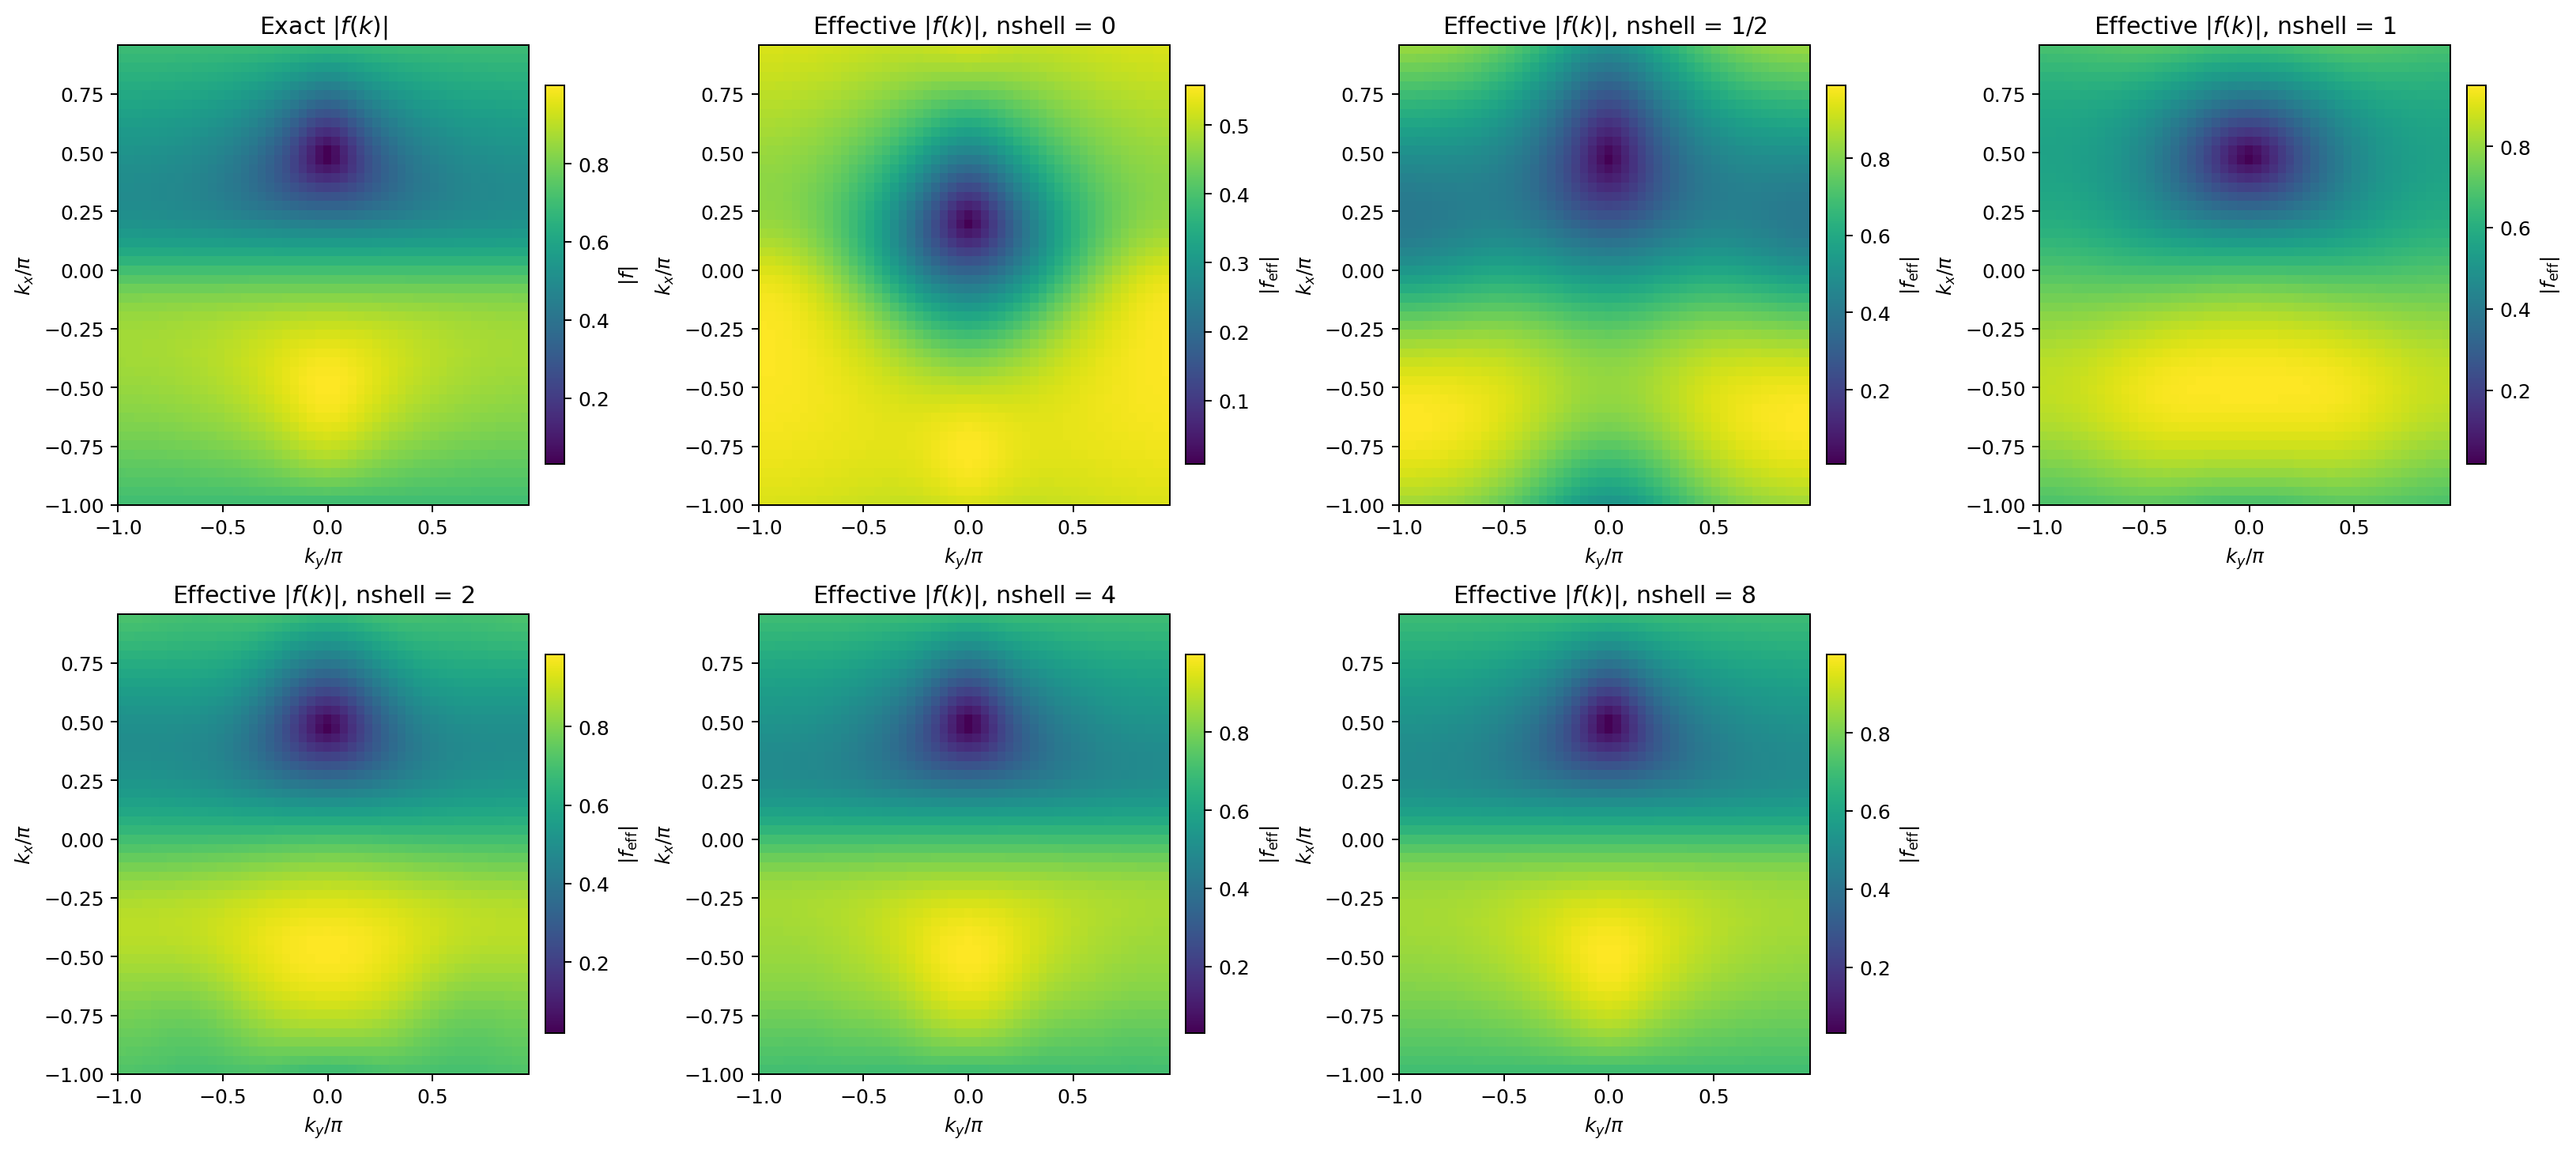
\includegraphics[width=\textwidth]{effective_form_factor_maps.png}
\caption{Momentum-space amplitude $|f_n^{\mathrm{eff}}(\mbf{k})|$ from the square real-space mask, for the exact unwindowed form factor (top left) and for $n_{\mathrm{shell}}=0,1/2,1,2,4,8$. Increasing $n_{\mathrm{shell}}$ concentrates the effective form factor amplitude toward the unwindowed result. Accidental shallow minima can appear for very small shells due to broad momentum mixing.}
\label{fig:effective-form-factor-maps}
\end{figure}

\begin{figure}[t]
\centering
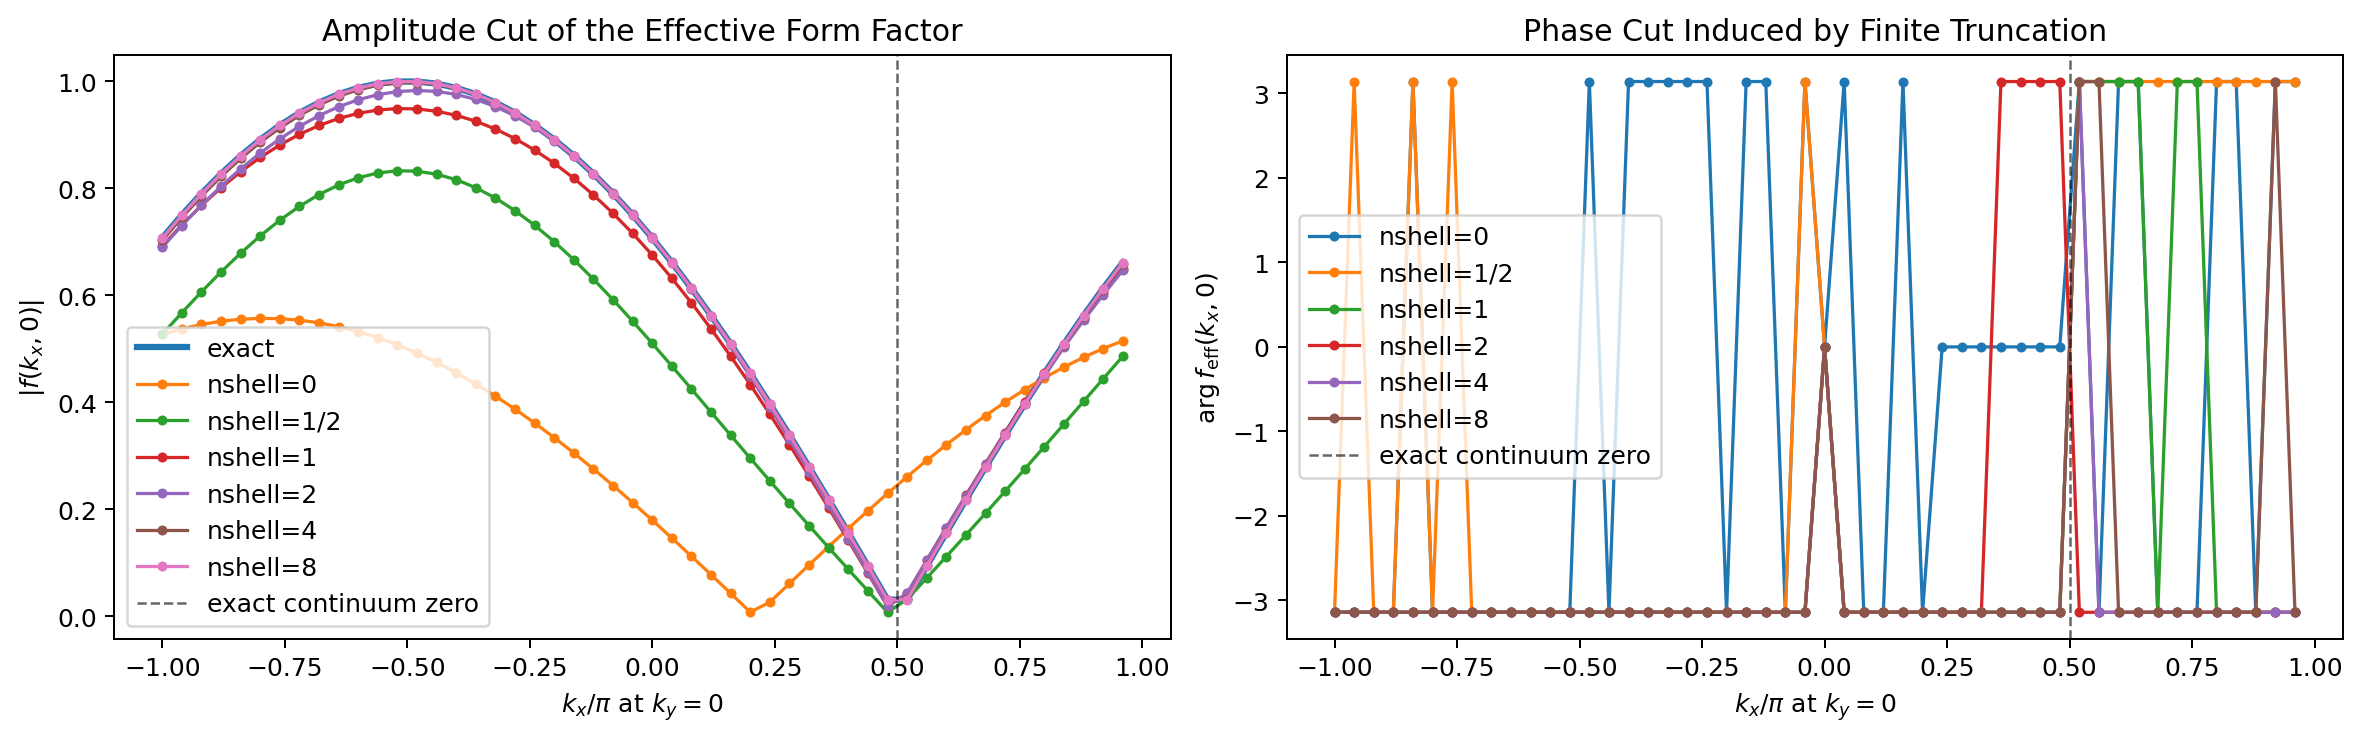
\includegraphics[width=\textwidth]{effective_form_factor_cuts.png}
\caption{Cuts at $k_y=0$ for the effective form factor amplitude (left) and phase (right), with momenta in units of $\pi$. The dashed vertical line marks the analytic continuum zero at $k_x/\pi=0.5$. The $n_{\mathrm{shell}}=0$ dip near $k_x/\pi\simeq 0.2$ is an accidental minimum, not the original topological zero.}
\label{fig:effective-form-factor-cuts}
\end{figure}

%%%%%%%%%%%%%%%%%%%%%%%%%%%%%%%%%%%%%%%%%%%%%%%%%%%%%
\section{Compact-Support Spinors and the FHS Diagnostic}
\label{sec:fhs}
%%%%%%%%%%%%%%%%%%%%%%%%%%%%%%%%%%%%%%%%%%%%%%%%%%%%%

The scalar form factor $f_n^{\mathrm{eff}}(\mbf{k})$ locates the obstruction encountered when the truncated OW mode is compared with the target lower band.  A different object is the normalized two-component trigonometric polynomial
\begin{equation}
\ket{\hat{\psi}_n(\mbf{k})} = \frac{\ket{\psi_n(\mbf{k})}}{\norm{\psi_n(\mbf{k})}},
\end{equation}
where $\ket{\psi_n(\mbf{k})}$ is defined in Eq.~\eqref{eq:spinor_continuum}.  If $\psi_n(\mbf{k})$ is nonzero throughout $T^2$, then it is itself a smooth periodic global section of the one-dimensional subspace spanned by $\hat{\psi}_n(\mbf{k})$.  Consequently,
\begin{equation}\label{eq:compact_global_section}
\psi_n(\mbf{k})\neq0\ \ \forall\,\mbf{k}\in T^2
\qquad\Longrightarrow\qquad
C_{\psi_n}=0 .
\end{equation}
This elementary global-section argument prevents one from identifying the winding of $\braket{u_-(\mbf{k})}{\psi_n(\mbf{k})}$ with a Chern number carried by a nonvanishing compact-support spinor.

For diagnostic purposes one may nevertheless apply the Fukui--Hatsugai--Suzuki (FHS) lattice discretization to $\hat{\psi}_n$:
\begin{equation}
C_{\psi_n}^{\mathrm{FHS}} = \frac{1}{2\pi}\sum_{\mbf{k}} F_{xy}(\mbf{k}),
\end{equation}
where
\begin{equation}
e^{iF_{xy}(\mbf{k})} = U_x(\mbf{k})\,U_y(\mbf{k}+\hat{x})\,U_x^*(\mbf{k}+\hat{y})\,U_y^*(\mbf{k}),
\qquad
U_\mu(\mbf{k}) = \frac{\braket{\hat{\psi}_n(\mbf{k})}{\hat{\psi}_n(\mbf{k}+\hat{\mu})}}{|\braket{\hat{\psi}_n(\mbf{k})}{\hat{\psi}_n(\mbf{k}+\hat{\mu})}|}.
\end{equation}
When $\norm{\psi_n}$ develops a very sharp but unresolved minimum, a coarse lattice evaluation can cross the admissibility boundary of the discrete formula and report a spurious nonzero integer.  Such an integer is not evidence for a nontrivial bundle unless convergence is established while the spinor remains resolved.

\subsection{Results for the square \texorpdfstring{$n_{\mathrm{shell}}$}{n-shell} mask}

\paragraph*{Target lower band.} The lower-band projector has nonzero Chern number, equivalently encoded by the overlap-form-factor zero at $\mbf{k}/\pi=(0.5,0)$.  This is the topological object probed by the OW measurement channel.

\paragraph*{Finite-support spinor.} For the compact-support fields computed from Eq.~\eqref{eq:spinor_continuum}, direct minimization of $\norm{\psi_n}$ and the stable FHS evaluation give
\begin{equation}
\begin{array}{c|c|c|c}
n_{\mathrm{shell}} & \min_{\mbf{k}}\norm{\psi_n(\mbf{k})} &
\nu_n\text{ of }f_n^{\mathrm{eff}} & C_{\psi_n}^{\mathrm{FHS}}\\
\hline
0   & 5.571\times10^{-1} & -1\ \text{(displaced accidental zero)} & 0\\
1/2 & 1.672\times10^{-1} & -1 & 0\\
1   & 5.106\times10^{-2} & -1 & 0\\
2   & 1.731\times10^{-2} & -1 & 0
\end{array}
\label{eq:fhs_corrected_table}
\end{equation}
Thus the $n_{\mathrm{shell}}=1$ overlap zero and winding are retained, while the compact-support spinor itself remains a globally defined trivial section.  For $n_{\mathrm{shell}}=4$ and $8$, the minimum norm becomes much smaller (approximately $2.05\times10^{-3}$ and $3.36\times10^{-5}$, respectively); nonzero FHS values on fixed coarse grids are therefore resolution-sensitive singular-limit diagnostics and are not used here to assign a Chern number to the finite-support spinor.

\paragraph*{Berry-flux maps.} Figure~\ref{fig:chern-surface-integral-flux} displays the finite-grid FHS flux diagnostic retained from the numerical study.  It visualizes concentration of discrete Berry flux as the compact-support spinor approaches an almost-zero.  It should not be read as replacing the overlap-winding test or overriding Eq.~\eqref{eq:compact_global_section}.

\begin{figure}[t]
\centering
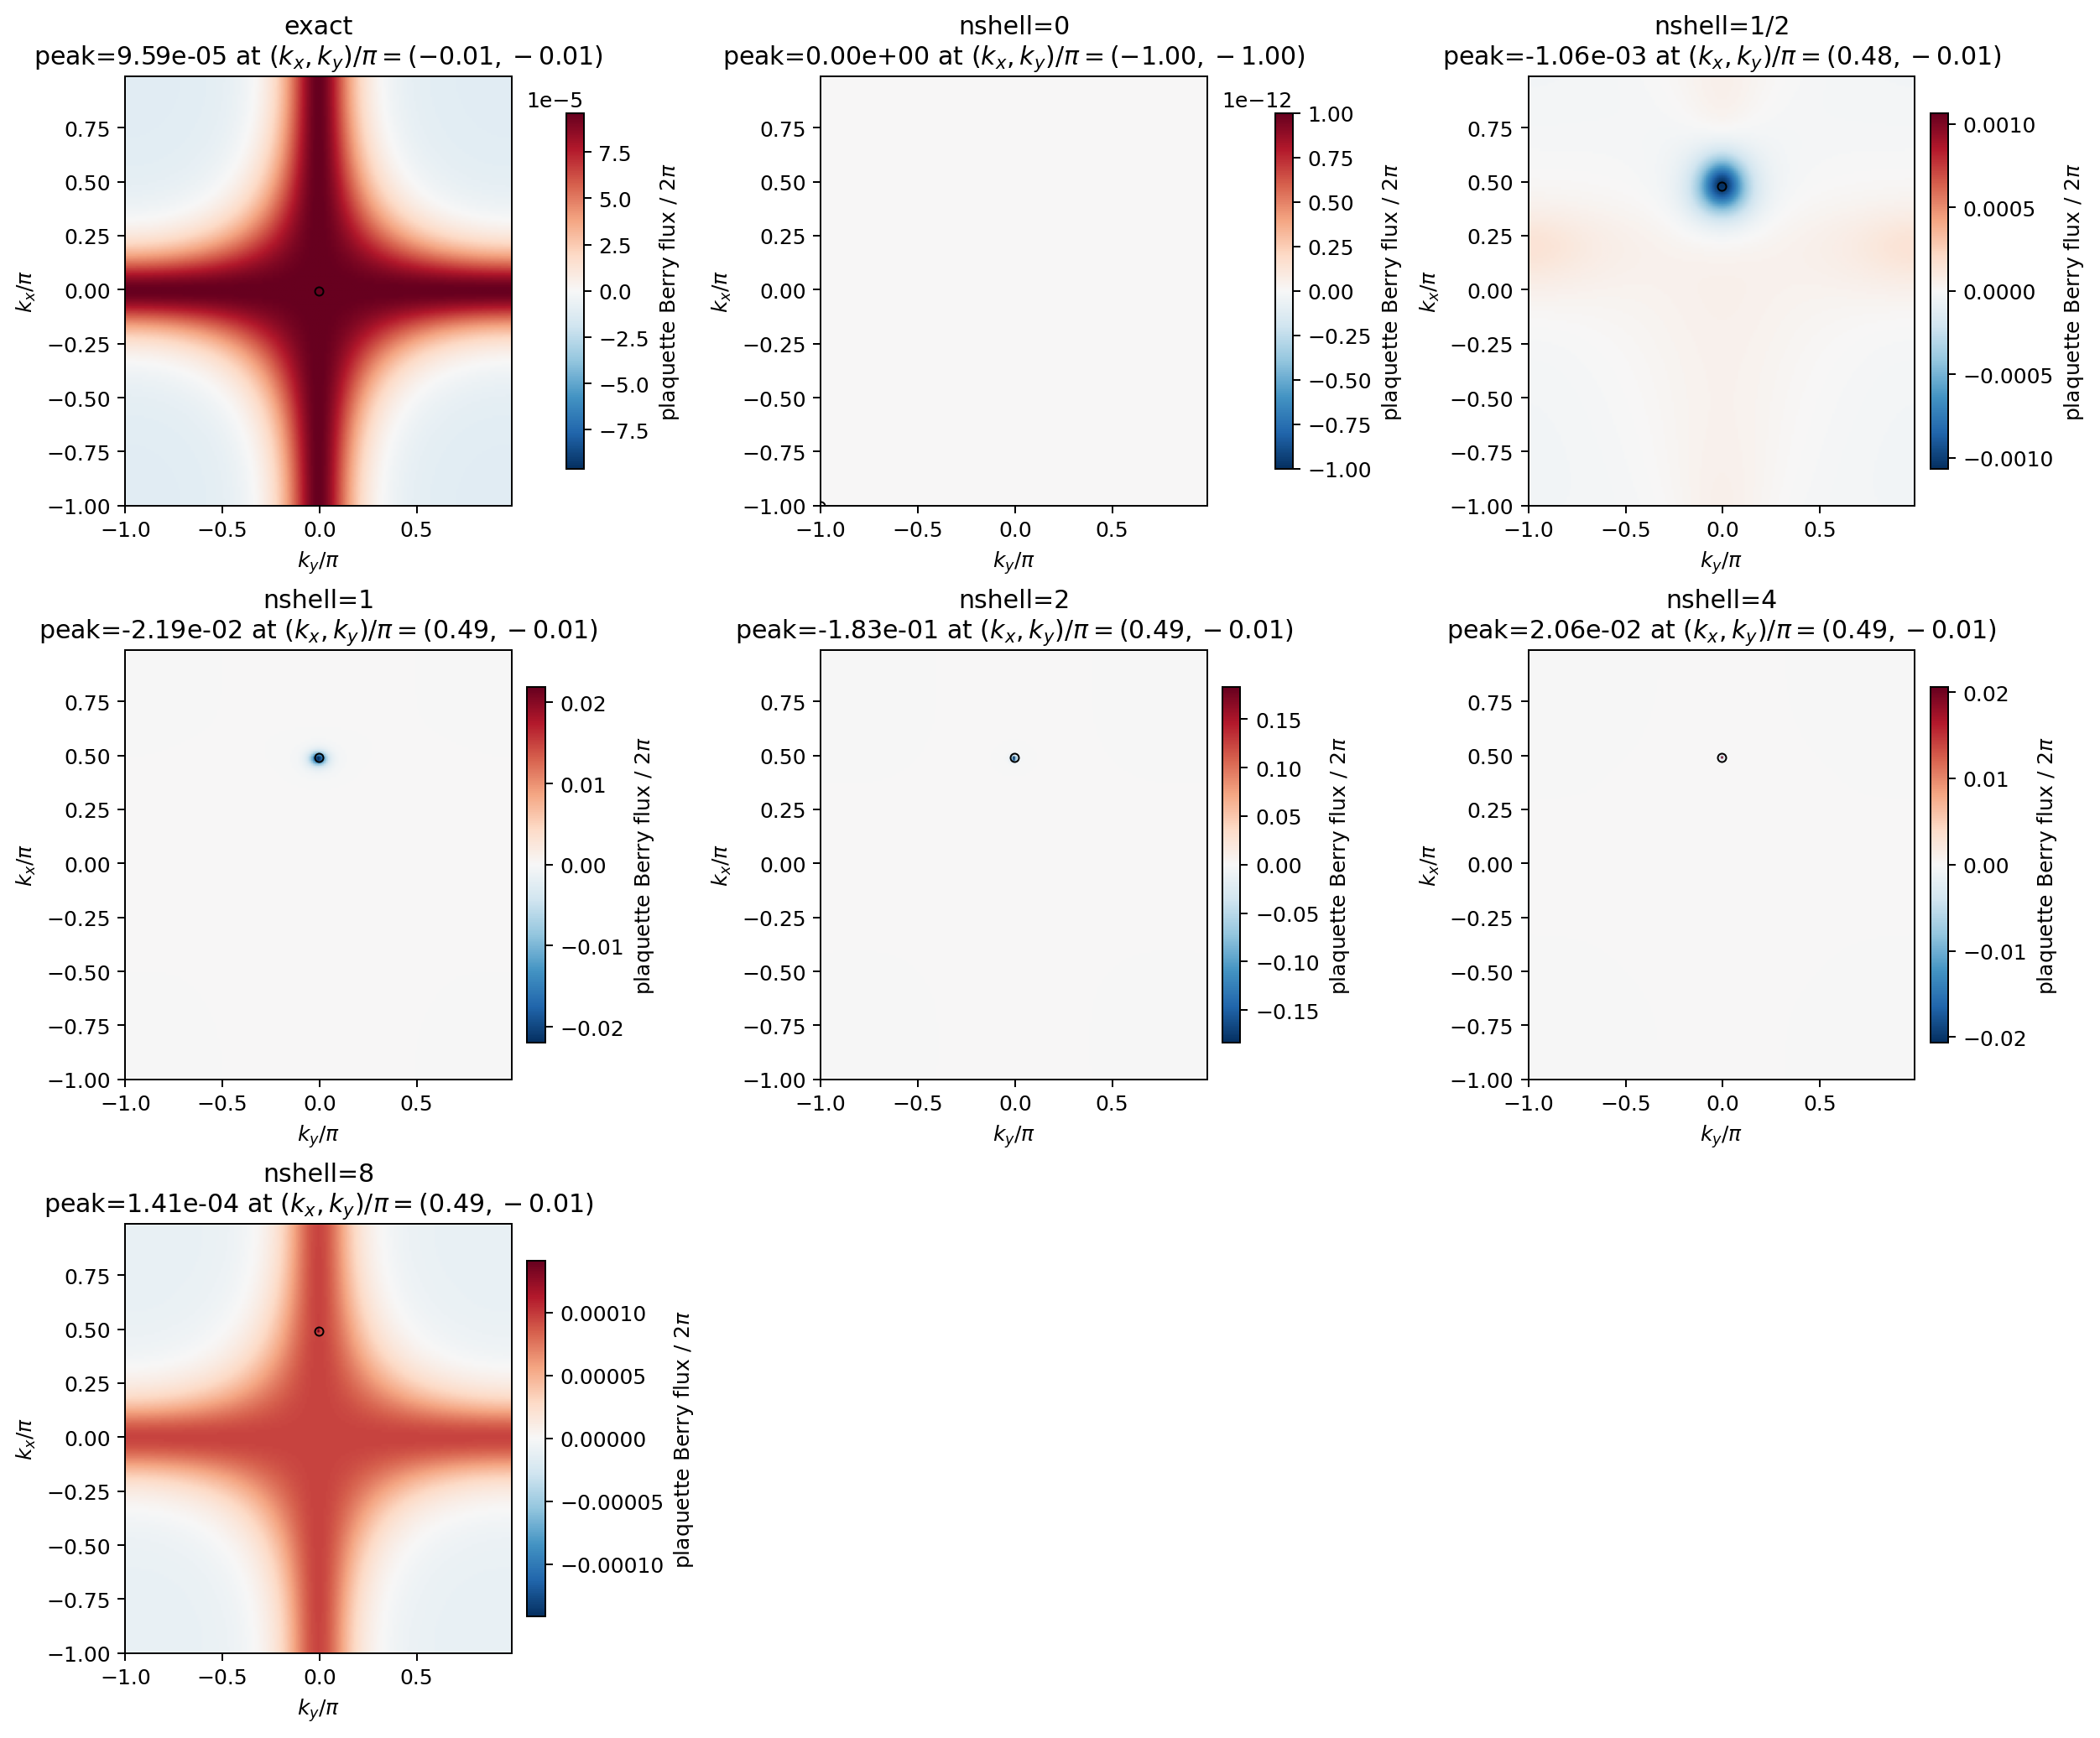
\includegraphics[width=\textwidth]{chern_surface_integral_flux_maps.png}
\caption{Finite-grid FHS Berry-flux diagnostic, $F_{xy}(\mbf{k})/(2\pi)$, for the target lower band and for the compact-support spinor $\ket{\psi_n(\mbf{k})}$.  As the minimum norm of the finite-support spinor becomes small, flux can concentrate within unresolved plaquettes and the discrete integer becomes grid-sensitive.  The topological circuit diagnostic used in this note is instead the zero and winding of $f_n^{\mathrm{eff}}$.}
\label{fig:chern-surface-integral-flux}
\end{figure}

\subsection{Distinction between overlap winding and compact-spinor Chern number}

Using the overlap-winding formula
\begin{equation}
\nu_n = \frac{1}{2\pi i}\oint d\mbf{k}\cdot\nabla_{\mbf{k}}\ln f_n^{\mathrm{eff}}(\mbf{k}),
\end{equation}
the contribution of each continuum zero is computed by integrating the phase of $f_n^{\mathrm{eff}}$ around a small loop enclosing that zero.  In the cases relevant to the circuit, the surviving $\nu_n=-1$ states that the finite-range measurement mode continues to encounter the lower-band Chern obstruction.  It does not assert that the standalone trigonometric-polynomial spinor $\psi_n$ is a nontrivial Bloch bundle.  This distinction is already visible at $n_{\mathrm{shell}}=0$, where a constant spinor has $C_{\psi_0}=0$ although its overlap with a nontrivial target band can possess a winding zero; it remains essential for all finite shells.

%%%%%%%%%%%%%%%%%%%%%%%%%%%%%%%%%%%%%%%%%%%%%%%%%%%%%
\section{Summary}
\label{sec:summary}
%%%%%%%%%%%%%%%%%%%%%%%%%%%%%%%%%%%%%%%%%%%%%%%%%%%%%

\begin{proposition}[Single band]\label{prop:single}
Let $\ket{\chi_{\mbf{R}}}$ be a coherent state in a band of Chern number $C \neq 0$, and let $g(\mbf{r})$ be an arbitrary complex-valued function on the lattice. Define the modulated state $\ket{\Phi^{(g)}} = g(\hat{\mbf{r}})\ket{\chi_{\mbf{R}}}$ and its effective form factor
\begin{equation}
f^{(g)}(\mbf{k}') = \frac{1}{N}\sum_{\mbf{k}} \tilde{g}(\mbf{k}'-\mbf{k})\,e^{-i(\mbf{k}'-\mbf{k})\cdot\mbf{R}}\, f(\mbf{k})\,\braket{u_{\mbf{k}'}}{u_{\mbf{k}}}.
\end{equation}
Then:
\begin{enumerate}
\item[(i)] \textbf{(Overlap criterion.)} The overlap-winding index $\nu_g=\frac{1}{2\pi i}\oint d\mbf{k}\cdot\nabla_{\mbf{k}}\ln f^{(g)}(\mbf{k})$ vanishes whenever $f^{(g)}$ is nowhere vanishing on $T^2$.
\item[(ii)] \textbf{(Preservation.)} If $\tilde{g}(\mbf{q})$ produces a sufficiently small perturbation on a loop surrounding an unwindowed zero, then $f^{(g)}$ inherits that zero's winding and $\nu_g=-C$.
\item[(iii)] \textbf{(Destruction.)} Sufficiently broad momentum mixing can remove the original overlap zero; if no replacement zero is generated, $\nu_g=0$.
\item[(iv)] \textbf{(Box window.)} For $\sigma\gg\xi_{\mathrm{rms}}$, the narrow-kernel/Rouch\'{e} argument protects overlap winding while allowing displacement of the zero.
\item[(v)] \textbf{(Length scales.)} The quantum-geometric inequality constrains $\xi_{\mathrm{rms}}\geq\xi_{\mathrm{top}}=\sqrt{2|C|}\,\ell$, whereas $\xi_{\mathrm{exp}}$ controls only the asymptotic real-space tail.
\item[(vi)] \textbf{(Compact spinor.)} If the finite-support spinor $\psi_n(\mbf{k})$ is smooth, periodic, and nowhere zero, then it is a global section and its own Chern number is zero, independently of $\nu_n$.
\end{enumerate}
\end{proposition}

\begin{proposition}[Multiband]\label{prop:multi}
Let $\ket{\chi_{m,\mbf{R}}}$, $m=1,\ldots,M$, be coherent states spanning an $M$-band subspace with total Chern number $C\neq 0$. Define the effective overlap matrix $F^{(g)}_{nm}(\mbf{k}')$ by \eqref{eq:Feff_general}. Then:
\begin{enumerate}
\item[(i$'$)] \textbf{(Overlap criterion.)} The determinant-overlap winding defined in Eq.~\eqref{eq:Cg_multi} vanishes when $\det F^{(g)}$ is nowhere zero.
\item[(ii$'$)] \textbf{(Preservation.)} A sufficiently gentle convolution preserves the determinant-zero winding of the target subspace.
\item[(iii$'$)] \textbf{(Interpretation.)} Without an in-subspace frame condition, $\nu_g^{(M)}$ is an overlap diagnostic and must not be automatically identified with a Chern invariant of the modulated vectors.
\item[(iv$'$)] \textbf{(Critical scale).} The parametric window scale is set by $\xi_{\mathrm{rms}}$, with $\xi_{\mathrm{rms}}\geq\sqrt{2|C|}\,\ell$.
\end{enumerate}
The key structural difference from the single-band case is that $\det F^{(g)}$ is a polynomial in the convolved matrix elements, so zeros can be created or annihilated in pairs at intermediate scales.
\end{proposition}

%%%%%%%%%%%%%%%%%%%%%%%%%%%%%%%%%%%%%%%%%%%%%%%%%%%%%
\section{Physical Interpretation and Circuit Implications}
\label{sec:physics}
%%%%%%%%%%%%%%%%%%%%%%%%%%%%%%%%%%%%%%%%%%%%%%%%%%%%%

\subsection{Topology stored in zero structure}

The Wannier obstruction of the target band is stored in the zeros of $f(\mbf{k})$, which are phase singularities carrying its overlap winding. Any real-space window acts as a momentum-space twisted convolution and may shift, create, or remove zeros of the overlap with that target band.  The RMS spread of the unwindowed OW mode is subject to a quantum-geometric lower bound, but neither that bound nor the exponential tail length alone determines the fate of a given discrete mask.  For the square mask the fate of the obstruction is resolved directly by the continuum form-factor cut.

\subsection{Universality of the criterion}

The general formula \eqref{eq:feff_general} makes clear that the overlap-zero structure depends on both the momentum-space width and the symmetry of $\tilde{g}$, as well as on the Bloch-overlap dressing.  Width compared with $1/\xi_{\mathrm{rms}}$ provides a controlled parametric guide for gentle windows; the explicit square-mask calculation is the relevant determination at small integer $n_{\mathrm{shell}}$.

\subsection{Implications for the adaptive Markov circuit}

In the adaptive circuit studied in the companion code, the OW measurement modes are constructed with a finite \texttt{nshell} cutoff: the Wannier mode centered at site $\mbf{R}$ is restricted to a $(2n+1)\times(2n+1)$ real-space patch. The analysis here shows that this truncation:
\begin{enumerate}
\item For $n_{\mathrm{shell}}=1$, the effective form factor $f_n^{\mathrm{eff}}(\mbf{k})$ has a zero with the inherited winding, displaced only slightly from the exact continuum location $\mbf{k}/\pi=(0.5,0)$.  It is therefore a compact finite-range measurement channel which still probes the Chern-band overlap obstruction.
\item At $\alpha=1$, the same $3\times3$ window retains $0.992155$ of the untruncated OW norm.  Its support radius is only comparable to the fitted tail scale $\xi_{\mathrm{exp}}\simeq1.443a$, so the decay length alone should be read only as supporting locality evidence, not as a proof that the topological zero survives.  The decisive check is the explicit continuum-$k$ square-mask calculation above: for $n_{\mathrm{shell}}=1$, $f_n^{\mathrm{eff}}(\mbf{k})$ retains the inherited overlap zero and winding.  Thus $n_{\mathrm{shell}}=1$ is justified by the combination of high retained norm and direct zero/winding survival, rather than by a several-correlation-length support criterion.
\item The finite-support spinor should not be assigned the Chern number of the target lower band merely from this overlap zero.  For the stable $n_{\mathrm{shell}}=1$ compact-spinor FHS check, $C_{\psi_1}^{\mathrm{FHS}}=0$, as required for a nonvanishing global section.
\end{enumerate}
The special case $n_{\mathrm{shell}}=0$ is qualitatively less faithful: its overlap zero is strongly displaced and arises even though its compact spinor is momentum independent.  For quantitative long-time observables, including the particle-transfer Lyapunov gap, comparison of $n_{\mathrm{shell}}=1$ against $n_{\mathrm{shell}}=2$ remains a useful convergence test; it is not required to establish survival of the form-factor winding.

The geometric scale $\xi_{\mathrm{top}}=a/\sqrt{\pi}\simeq0.564a$ gives a lower bound on the RMS size of an OW mode in the \(\alpha=1\), \(|C|=1\) band.  It is not a certification radius for a discrete truncation.  The justification for $n_{\mathrm{shell}}=1$ is instead the direct combination of high retained norm and the explicitly preserved overlap zero.

\begin{acknowledgments}
This working note accompanies the adaptive class-A Markov circuit project. The analysis builds on the overcomplete Wannier framework of Li, Dong, Ledwith, and Khalaf \cite{Li2024}.
\end{acknowledgments}

\begin{thebibliography}{9}
\bibitem{Li2024} Q.~Li, J.~Dong, P.~J.~Ledwith, and E.~Khalaf, arXiv:2407.02561 (2024).
\bibitem{Fukui2005} T.~Fukui, Y.~Hatsugai, and H.~Suzuki, J.~Phys.~Soc.~Jpn.~\textbf{74}, 1674 (2005).
\end{thebibliography}

\end{document}
